\author{João Gonçalves}
\newcommand{\authorr}{Teresa Nogueira}
\newcommand{\studentID}{99995}
\newcommand{\studentIDD}{100029}
%\newcommand{\supervisorone}{Prof\textsuperscript{\underline{a}}. XXXXXX}
\newcommand{\supervisorone}{}
\newcommand{\supervisortwo}{}
\newcommand{\department}{Engenharia Eletrotécnica e de Computadores}
\newcommand{\exam}{Telecomunicações}

\title{%
Apontamentos \\
\large (Alguns tópicos \href{https://github.com/Kons-5}{\raisebox{0 em}{\large \faGithub}})}
\date{Janeiro 2023}

\documentclass[a4paper,12pt]{article}
\usepackage[left=28mm,top=25mm,right=28mm,bottom=24mm]{geometry}
\usepackage[flushmargin,hang,bottom,multiple]{footmisc}
\usepackage{etoolbox}
\usepackage{fontawesome5}
\usepackage{pgfplots}
\usepackage{circuitikz}
\usepackage{booktabs}
\usepackage[usestackEOL]{stackengine}
\usepackage[T1]{fontenc}
\usepackage[utf8]{inputenc}
\usepackage{bm}
\usepackage[export]{adjustbox}
\usepackage{graphicx}
\usepackage[font=footnotesize]{caption}
\usepackage[justification=centering]{subcaption}
\usepackage{amsmath}
\usepackage{amsfonts}
\usepackage{mathtools}
\usepackage{float}
\usepackage[linktoc=all]{hyperref}
\usepackage[capitalise]{cleveref}
\usepackage{enumitem,kantlipsum}
\usepackage[square,numbers,sort]{natbib}
\usepackage[ruled,vlined]{algorithm2e}
\usepackage{listings}
\usepackage[numbered,framed]{matlab-prettifier}
\usepackage{minted}
\usepackage{amssymb}
\usepackage{babel}
\usepackage[nottoc,numbib]{tocbibind}
\usepackage{tcolorbox}
\usepackage{xcolor}
\usepackage{graphicx,array}
\usepackage{animate}
\usepackage{breakurl}
\usepackage{placeins}
\usepackage{colortbl}
\usepackage{attrib}
\usepackage{wrapfig}
\usepackage{mathabx}
\usepackage{fancyhdr}
\usepackage{amsmath}
\usepackage{lipsum}
\usepackage{textcomp}
\usepackage{physics}
\usepackage{cancel}
\usepackage[printwatermark]{xwatermark}
\usepackage[framemethod=TikZ]{mdframed}
%\tcbuselibrary{skins,breakable}
%\usetikzlibrary{shadings,shadows}
\usemintedstyle{emacs}
\linespread{1}
%\setlength{\parindent}{0pt}

\usepackage{multimedia}

\newenvironment{block}[1]{%
    \tcolorbox[beamer,%
    noparskip,breakable,
    colback=LightBlue,colframe=DarkBlue,%
    colbacklower=DarkBlue!75!LightBlue,%
    title=#1]}%
    {\endtcolorbox}

\hypersetup{
    colorlinks,
    linkcolor={black},
    citecolor={blue!50!black},
    urlcolor={blue!50!black}
}

\lstset{
  style              = Matlab-editor,
  basicstyle         = \scriptsize\mlttfamily,
  escapechar         = ",
  mlshowsectionrules = true,
  extendedchars=true,
  literate= {á}{{\'a}}1 {é}{{\'e}}1 {í}{{\'i}}1 {ó}{{\'o}}1 {ú}{{\'u}}1 {ç}{{\c c}}1 {ã}{{\~a}}1 {õ}{{\~o}}1
  {Á}{{\'A}}1 {É}{{\'E}}1 {Í}{{\'I}}1 {Ó}{{\'O}}1 {Ú}{{\'U}}1 {Ã}{{\~A}}1,
}

%//==============================--@--==============================//%
%                         -> error messages <-                        %
\usepackage{pifont}

\newenvironment{warning}
  {\par\begin{mdframed}[linewidth=1.5pt,linecolor=red]%
    \begin{list}{}{\leftmargin=0.9cm
                   \labelwidth=\leftmargin}\item[\raisebox{-0.4 em}{\Large\ding{43}}]}
  {\end{list}\end{mdframed}\par}

%//==============================--@--==============================//%
%                   -> reduzir espaço entre itens <-                  %
\usepackage{enumitem}
%\setlist[itemize]{nosep}
%\setlist[enumerate]{nosep}
\setlist[itemize]{itemsep=0.0125em}
\setlist[enumerate]{itemsep=0.0125em}
%//==============================METH-==============================//%
\newcounter{theo}[section]\setcounter{theo}{0}
\renewcommand{\thetheo}{\arabic{theo}}

%\definecolor{tempcolor}{RGB}{113, 110, 97}
\definecolor{tempcolor}{RGB}{0, 0, 0}
\newenvironment{theo}[2][]{%
    \refstepcounter{theo}
    \ifstrempty{#1}%
    % if condition (without title)
    {\mdfsetup{%
        frametitle={%
            \tikz[baseline=(current bounding box.east),outer sep=0pt]
            \node[anchor=east,rectangle,fill=blue!20]
            {\strut Teorema~\thetheo};}
        }%
    % else condition (with title)
    }{\mdfsetup{%
        frametitle={%
            \tikz[baseline=(current bounding box.east),outer sep=0pt]
            \node[anchor=east,rectangle,fill=white]
            {\strut #1};}%
        }%
    }%
    % Both conditions
    \mdfsetup{%
        innertopmargin=0pt,linecolor=tempcolor,%
        linewidth=2pt,topline=true,%
        frametitleaboveskip=1.25\dimexpr-\ht\strutbox\relax%
    }
 
\begin{mdframed}[]\relax\vspace{-0.5em}}{%
\end{mdframed}}

\def\delequal{\mathrel{\ensurestackMath{\stackon[1pt]{=}{\scriptstyle\Delta}}}}

\let\originalleft\left
\let\originalright\right
\renewcommand{\left}{\mathopen{}\mathclose\bgroup\originalleft}
\renewcommand{\right}{\aftergroup\egroup\originalright}
%------------------------------------ MAGIC--------------------------------------
\def\UrlBreaks{\do\/\do-}
\expandafter\def\expandafter\UrlBreaks\expandafter{\UrlBreaks\do\a%
\do\b\do\c\do\d\do\e\do\f\do\g\do\h\do\i\do\j\do\k\do\l\do\m\do\n%
\do\o\do\p\do\q\do\r\do\s\do\t\do\u\do\v\do\w\do\x\do\y\do\z\do\&}

\newcolumntype{C}[1]{>{\centering\let\newline\\\arraybackslash\hspace{0pt}}m{#1}}
\newcolumntype{L}[1]{>{\raggedright\let\newline\\\arraybackslash\hspace{0pt}}m{#1}}
%----------------------------------TITLE PAGE -----------------------------------
\makeatletter
\def\maketitle{
  \begin{center}\leavevmode
        \normalfont
        
\includegraphics[width=0.5\columnwidth]{img/title-page/IST.pdf}
        \vskip 0.05cm   
        \textsc{\large \department}\\
        \vskip 0.5cm
        \rule{0.95\linewidth}{0.2 mm} %\\
        {\large \exam}\\[0.5 cm]
        {\huge \bfseries \@title \par} 
        \vspace{1em}
        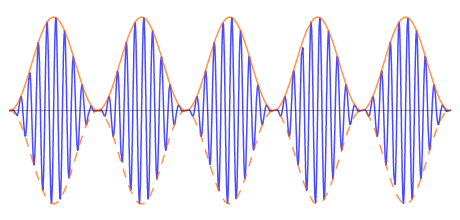
\includegraphics[scale=0.7]{img/title-page/000.png}
        \vspace{-0.5em}
        \captionof*{figure}{\color{gray} Imagem: \textit{Illustration of the envelope}}
        %\vspace{0.5cm}
        \rule{0.95\linewidth}{0.2 mm} \\[0.75 cm]
        %\fontsize{9pt}{11pt}\selectfont
        \begin{minipage}[t]{1\textwidth}
	   \begin{flushleft} \large
                \emph{Autores:}\\
			\normalsize \textbf{\@author} : \studentID\\
                \fontsize{9pt}{11pt}\selectfont $\hookrightarrow$ jrazevedogoncalves@tecnico.ulisboa.pt \\
                \normalsize \textbf{\authorr} : \studentIDD\\
                \scriptsize $\hookrightarrow$ maria.teresa.ramos.nogueira@tecnico.ulisboa.pt
		\end{flushleft}
	\end{minipage}
	\vfill
	{\Large \@date\par}
   \end{center}
   %\vfill
   %\null
   \cleardoublepage
  }
\makeatother
%-------------------------------- ENDTITLE PAGE ----------------------------------
%---> Header <---
%\fancyhf{}
\renewcommand{\headrulewidth}{1pt}% Header rule width
\renewcommand{\footrulewidth}{0pt}% No footer rule
\setlength\headheight{26pt} 
\fancyhead[L]{\raisebox{0.1\height}[0pt][0pt]{\textit{Telecomunicações}}}
\fancyhead[R]{\raisebox{0.1\height}[0pt][0pt]{2022/2023}}

\pgfplotsset{compat=1.18}
\setcounter{tocdepth}{4}
%\setcounter{secnumdepth}{4}
\setcounter{secnumdepth}{-2}

\renewcommand{\figurename}{Fig.}
\renewcommand{\tablename}{Tab.}
\renewcommand{\contentsname}{Índice}
\settocbibname{\raisebox{0em}{Referências}}
\setlength{\bibsep}{0.1em}%reduzir espaço entre refs.

%\renewcommand{\bibpreamble}{\vspace{-8em}}
\usepackage[titles]{tocloft}
\setlength{\cftbeforesecskip}{0.25em}

%\usepackage{pdfpages}
\newwatermark[page=15,fontfamily=bch,color=red!50,angle=45,scale=3.5,xpos=-10,ypos=10]{TO BE ADDED}


\begin{document}
    \sloppy
    %% title page
    \pagenumbering{gobble}
    \maketitle
    %% toc
    \tableofcontents
    %% body
    \newpage
    \pagestyle{fancy}
    \pagenumbering{arabic}
    % %\phantomsection\addcontentsline{toc}{section}{}\vskip -0em%
    %     \input{src/Intro}

    \setlength{\abovedisplayskip}{3pt}
    \setlength{\belowdisplayskip}{3pt}
    \setlength{\fboxsep}{1.25\fboxsep}

    \let\zzzfootnotesize\footnotesize
    \def\newfootnotesize{%
    \zzzfootnotesize
    \abovedisplayskip=0pt
    \belowdisplayskip=\abovedisplayskip
    \abovedisplayshortskip=\abovedisplayskip
    \belowdisplayshortskip=\abovedisplayskip
    }
    \renewcommand\footnotesize{\protect\newfootnotesize}
    
    \mdfsetup{%
        linewidth=2pt
    }

    \clearpage
    \section{1. Conceitos gerais}
        %//==============================--@--==============================//%
\subsection{1.1 Classificação de sinais}
\label{subsec:signal-classification}

\begin{mdframed}
    \begin{enumerate}[leftmargin=2em]
        \item[$\pmb{\star}$] Um sinal $x(t)$ diz-se \textit{deterministico} se, $\forall t$, o valor de $x(t)$ é real ou complexo.
        \item[$\pmb{\star}$] Um sinal $x(t)$ diz-se \textit{aleatório} ou \textit{estocástico} se, $\forall t$, o valor de $x(t)$ é uma variável aleatória; isto é, é definido por uma função densidade de probabilidade.
        \item[$\pmb{\star}$] Um sinal $x(t)$ diz-se periódico se verificar:
        $$
            x(t+kT) = x(t),\quad \forall t \in \mathbb{R},\quad \forall k \in \mathbb{Z}
        $$
        onde $T$ é definido como o período do sinal. Um sinal que não verifique esta propriedade, diz-se \textit{aperiódico}.
        \item[$\pmb{\star}$] Um sinal diz-se um \textit{sinal de energia} se a sua energia
        $$
            E_x = \int_{-\infty}^{+\infty} \left| x(t) \right|^2\, dt
        $$
        for finita.
        \item[$\pmb{\star}$] Um sinal diz-se um \textit{sinal de potência} se a sua potência
        $$
            P_x = \lim_{L \to +\infty} \frac{1}{L} \int_{-L/2}^{+L/2} \left| x(t) \right|^2\, dt
        $$
        for finita. Para um sinal periódico $x(t)$, de período $T$, a potência é dada por:
        $$
            P_x = \lim_{n\to +\infty} \frac{E_x}{nT} = \frac{1}{T} \int_{T} \left| x(t) \right|^2\, dt
        $$
    \end{enumerate}
\end{mdframed}

%//==============================--@--==============================//%
\subsubsection{1.1.1 Alguns sinais importantes}
\label{subsubsec:some-important-signals}

\begin{mdframed}
    \begin{enumerate}[leftmargin=2em]
        \item[$\pmb{\star}$] \textbf{Sinal sinusoidal:}
            $$
                x(t) = A \cos{(2\pi f_0 t + \theta)}
            $$
        É um sinal com potência dada por $P_x = A^2/2$.
        \item[$\pmb{\star}$] \textbf{Pulso rectangular:}
            $$
                x(t) = \text{rect}(\frac{t-t_0}{T}) = \Pi(\frac{t-t_0}{T}) \delequal
                \begin{cases}
                    1 & \text{se}\, \left| t-t_0 \right| \leq T/2 \\
                    0 & \text{se}\, \left| t-t_0 \right| > T/2
                \end{cases}
            $$
        É um sinal com energia dada por $E_x = T$.
        \item[$\pmb{\star}$] \textbf{Pulso triangular:}
            $$
                x(t) = \text{tri}(\frac{t-t_0}{T}) = \Lambda(\frac{t-t_0}{T}) \delequal
                \begin{cases}
                    1 - \left|t-t_0\right|/T & \text{se}\, \left| t-t_0 \right| \leq T/2 \\
                    0 & \text{se}\, \left| t-t_0 \right| > T/2
                \end{cases}
            $$
        É um sinal com energia dada por $E_x = 2T/3$.
        \item[$\pmb{\star}$] \textbf{Sinal sinc\footnotemark[1]:}
            $$
                x(t) = \text{sinc}(t) \delequal 
                \begin{cases}
                    \sin(\pi t)/\pi t & \text{se}\; t \neq 0\\
                    1 & \text{se}\; t = 0
                \end{cases}
            $$
        É um sinal de energia unitária, i.e., $E_x = 1$.
    \end{enumerate}
\end{mdframed}

\footnotetext[1]{Alguns livros definem uma função similar: $\text{Sa}(t) \delequal \sin(t)/t$, desta forma, $\text{sinc}(t) = \text{Sa}(\pi t)$.}

\noindent $\pmb{\star}$ \textbf{Sinal delta ou impulso de Dirac:}

\noindent Relembrando Sinais e Sistemas, $\delta(t)$ é uma função generalizada que pode ser definida por (\textit{sifting property}):
$$
    \int_{\mathbb{R}} x(t)\delta(t-t_0) = x(t_0)
$$
(Para $x(t) \equiv 1$, verifica $\int_{\mathbb{R}} \delta(t-t_0) = 1$).
\\\\
Uma dilatação ou contração temporal, resulta em:
$$
    \delta(at) = \frac{1}{|a|}\delta(t), \qquad a \in \mathbb{C}
$$
O integral do impulso de Dirac é o degrau unitário:
$$
    u(t) \delequal \int_{-\infty}^{t} \delta(\lambda)\, d\lambda =
    \begin{cases}
        0 & \text{se}\; t < 0 \\
        1 & \text{se}\; t > 0
    \end{cases}
$$
Dualmente, a derivada do degrau unitário é:
$$
    \frac{d u(t)}{dt} \delequal \delta(t)
$$

%//==============================--@--==============================//%
\subsubsection{1.1.2 Correlação de sinais}
\label{subsubsec:correlation-of-two-signals}

A correlação (\textit{cross-correlation}) de dois sinais, $x(t)$ e $y(t)$, é dada por:
$$
    R_{xy}(\tau) \delequal \int_{\mathbb{R}} x(t)y^{*}(t-\tau)\, dt
$$
É uma medida da similaridade entre sinais. 

Caso $x(t) = y(t)$, define-se a função de autocorrelação:
$$
    R_{x}(\tau) \delequal \int_{\mathbb{R}} x(t)x^{*}(t-\tau)\, dt
$$
Particularmente, se $\tau = 0$ verifica-se $\rightarrow R_{x}(\tau = 0) = E_x$. 

\vspace{-1em}
\noindent{\begin{center}\rule{8cm}{1pt} \end{center}} 

\vspace{-0.5em}
\noindent Dado um sinal de potência $z(t)$, define-se a sua média temporal como:
$$
    \left<z(t)\right>\;\, \delequal \lim_{L\to +\infty} \frac{1}{L} \int_{-L/2}^{L/2} z(t)\, dt 
$$
Define-se então, a correlação entre dois sinais de potência, $x(t)$ e $y(t)$, como 
$$
    R_{xy}(\tau) =\;\, \left<x(t)y^{*}(t-\tau)\right>\;\, \delequal \lim_{L\to +\infty} \frac{1}{L} \int_{-L/2}^{L/2} x(t)y^{*}(t-\tau)\, dt 
$$
Novamente, no caso particular em que $x(t) = y(t)$, obtemos a função de autocorrelação:
$$
    R_{x}(\tau) =\;\, \left<x(t)x^{*}(t-\tau)\right>\;\, \delequal  \lim_{L\to +\infty} \frac{1}{L} \int_{-L/2}^{L/2} x(t)x^{*}(t-\tau)\, dt 
$$
Quando $x(t)$ é periódico com período $T$, temos
$$
    R_{x}(\tau) \delequal \frac{1}{T} \int_{T} x(t)x^{*}(t-\tau)\, dt 
$$

\noindent A função de autocorrelação de sinais de energia $[$potência$]$ (reais) verifica:
\begin{enumerate}\footnotesize
    \item[$\pmb{\star}$] $R_x(\tau = 0) = S$, onde $S$ representa a energia $[$potência média$]$ do sinal $x(t)$.
    \item[$\pmb{\star}$] $R_x(0) \ge R_x(\tau)$.
    \item[$\pmb{\star}$] $R_x(-\tau) = R_x(\tau)$, a autocorrelação é uma função par. 
\end{enumerate}

%//==============================--@--==============================//%
\newpage
\subsection{1.2 Análise de Fourier}
\label{subsec:fourier-analysis}

\begin{theo}[\underline{Séries de Fourier}]{def:fourier-series}\label{def:fourier-series}
    Seja $x(t)$ um sinal periódico, de período $T$, que verifica as \underline{condições de Dirichlet}:
    
    \vspace{-0.75em}
    \begin{enumerate}[leftmargin=2em]
        \item[$\pmb{1.}$] $x(t)$ é absolutamente integrável num intervalo correspondente a um período:
        $$
            \int_T \left|x(t)\right|\, dt < +\infty
        $$
        \item[$\pmb{2.}$] O número de máximos e mínimos de $x(t)$ num intervalo $T$, \underline{é finito}.
        
        \item[$\pmb{3.}$] O número de descontinuidades de $x(t)$ em cada intervalo, \underline{é finito}.
    \end{enumerate}

    \noindent Satisfazendo estas condições, define-se a Série de Fourier correspondente ao sinal $x(t)$ como
    $$
        \boxed{\tilde{x}(t) = \sum_{n=-\infty}^{+\infty} c_n e^{j2\pi n f_0 t},\quad f_0 \delequal \frac{1}{T}}
    $$
    onde
    $$
    \tilde{x}(t) =
    \begin{cases}
        x(t) & \text{se $x(t)$ for continuo em $t$} \\
        \frac{x(t^-) + x(t^+)}{2} & \text{se $x(t)$ for descontinuo em $t$.}
    \end{cases}
    $$
    Os coeficientes da Série de Fourier são dados por
    $$
        c_n = \frac{1}{T} \int_T x(t) e^{-j 2\pi n f_0 t}\, dt
    $$

    \vspace{0.5em}
    \noindent $\pmb{\rightarrow}$ \textbf{Nota:} Se $x(t)$ é real, então \underline{$c_{-n} = c_{n}^*$}, e segue que: 
    
    \vspace{-0.75em}
    \begin{enumerate}[leftmargin=2em]
        \item[$\pmb{\star}$] Se $x(t)$ for \underline{real e par}, então os coeficientes são todos reais $\rightarrow$ $c_{-n} = c_{n}$. 
        
        \item[$\pmb{\star}$] Se $x(t)$ for \underline{real e ímpar}, então os coeficientes são imaginários $\rightarrow$ $c_{-n} = -c_{n}$.
    \end{enumerate}
\end{theo}

%\newpage
\begin{theo}[\underline{Transformada de Fourier}]{def:fourier-transform}\label{def:fourier-transform}
    Seja $x(t)$ um sinal que verifica as \underline{condições de Dirichlet}:
    
    \vspace{-0.5em}
    \begin{enumerate}[leftmargin=2em]
        \item[$\pmb{1.}$] $x(t)$ é absolutamente integrável na linha dos reais:
        $$
            \int_{\mathbb{R}} \left|x(t)\right|\, dt < +\infty
        $$
        \item[$\pmb{2.}$] O número de máximos e mínimos de $x(t)$ em qualquer intervalo finito, \underline{é finito}.
        
        \item[$\pmb{3.}$] O número de descontinuidades de $x(t)$ em qualquer intervalo finito, \underline{é finito}.
    \end{enumerate}

    \noindent Define-se o par de equações relativo à Transformada de Fourier de $x(t)$ como
    \begin{align*}
        X(f) = \mathcal{F}\{x(t)\} &\delequal \int_{\mathbb{R}} x(t) e^{-j2\pi ft}\, dt & \text{\underline{Equação de análise}}\\
        x(t) = \mathcal{F}^{-1}\{X(f)\} &\delequal \int_{\mathbb{R}} X(f) e^{j2\pi ft}\, df & \text{\underline{Equação de síntese}}
    \end{align*}%hewo :3  adoro-te totalmente

    \vspace{0.5em}
    \noindent $\pmb{\rightarrow}$ \textbf{Nota:} $X(f)$ é denominado por espectro de $x(t)$.
\end{theo}

\begin{theo}[\underline{Relação entre a Série e a Transformada de Fourier}]{def:fourier-relation}\label{def:fourier-relation}
\noindent Se $\tilde{x}(t)$ for a extensão periódica de $x(t)$ (truncado, ou absolutamente integrável---como um pulso), com período $T$, os coeficientes da sua Série de Fourier, $c_n$, relacionam-se com a Transformada de Fourier de $x(t)$:
    $$
        c_n = \frac{1}{T} X(nf_0)
    $$
    A Transformada de Fourier de um sinal periódico é: 
    $$
        \tilde{X}(f) = \sum_{n=-\infty}^{+\infty} c_n \delta(f - n f_0)
    $$
\end{theo}

%//==============================--@--==============================//%
\subsection{1.3 Teoremas de Wiener–Khinchin, Rayleigh e de Parseval}
\label{subsec:wierner-khinchin-parseval}

\begin{theo}[\underline{Teorema da Energia de Rayleigh} (Teorema de Parseval)]{def:parseval-rayleigh}\label{def:parseval-rayleigh}
    $$
        E_x = \int_{\mathbb{R}} \left| x(t) \right|^2\, dt = \int_{\mathbb{R}} \left| X(f) \right|^2\, df = \int_{\mathbb{R}} \psi_x(f)\, df
    $$
    ``(...) the total energy of a Fourier-transformable signal equals the total area under the curve of squared amplitude spectrum of this signal.''\cite{Haykin2007}

    \noindent $\pmb{\star}$ A quantia $\psi_x(f) \delequal \left| X(f) \right|^2$ é denominada por \textit{densidade espectral energética} ou \textit{espectro energético} de $x(t)$.
\end{theo}

\begin{theo}[\underline{Teorema de Parseval} (da potência)]{def:parseval-power}\label{def:parseval-power}
    Para sinais periódicos que podem ser representados sobre uma Série de Fourier, existe uma relação para a potência entre o domínio do tempo e da frequência.
    $$
        P_x = \frac{1}{T} \int_{T} \left| x(t) \right|^2 = \sum_{n=-\infty}^{+\infty} \left| c_n \right|^2
    $$
    em que $c_n$ são os coeficientes da Série de Fourier complexa.
\end{theo}

\begin{theo}[\underline{Teorema de Wiener-Khinchin}]{def:wierner-khinchin}\label{def:wierner-khinchin}
    $$
        S_x(f) = \int_{\mathbb{R}} R_x(\tau)\, e^{-j2\pi f \tau}\, d\tau 
        \quad \land \quad 
        R_x(\tau) = \int_{\mathbb{R}} S_x(f)\, e^{j2\pi f \tau}\, df
    $$

    \noindent Para sinais de energia:
    \begin{align*}
        \psi_x(f) &= \mathcal{F}\{R_x(\tau)\} = \int_{\mathbb{R}} R_x(\tau)\, e^{-j2\pi f \tau}\, d\tau \\
        R_x(\tau) &= \mathcal{F}^{-1}\{\psi_x(f)\} = \int_{\mathbb{R}} \psi_x(f)\, e^{j2\pi f \tau}\, df
    \end{align*}

    \noindent Para sinais periódicos que podem ser desenvolvidos numa Série de Fourier:
    \begin{align*}
        S_x(f) &= \mathcal{F}\{R_x(\tau)\} = \sum_{n=-\infty}^{+\infty} \left| c_n \right|^2 \delta(f-nf_0) \\
        R_x(\tau) &= \mathcal{F}^{-1}\{S_x(\tau)\}
    \end{align*}

    \vspace{0.25em}
    \noindent $\pmb{\rightarrow}$ \textbf{Nota:} $S_x(f)$ é a \textit{densidade espectral de potência} de $x(t)$; indica a distribuição da potência do sinal ao longo do domínio da frequência.
\end{theo}
%//==============================--@--==============================//%
        %//==============================--@--==============================//%
\subsection{1.4 Processos estocásticos (ou aleatórios)}
\label{subsec:stochastic-processes}
%//==============================--@--==============================//%
\subsubsection{1.4.1 Estatísticas}
\paragraph[1.4.1.1 Valor médio]{$\pmb{\star}$ Valor médio}\mbox{}\\
O valor médio de $X(t)$ é definido por
$$
    \mu_x(t) \delequal \mathbb{E}[X(t)] = \int_{\mathbb{R}} x f_{X(t)}(x)\,dx
$$
e é, com generalidade, uma função do tempo.
%//==============================--@--==============================//%
\paragraph[1.4.1.2 Função de autocorrelação]{$\pmb{\star}$ Função de autocorrelação}\mbox{}\\
A função de autocorrelação é definida por
$$
    R_x(t_1, t_2) \delequal \mathbb{E}[X(t_1)X(t_2)] = \int_{\mathbb{R}^2} x_1 x_2\, f_{X(t_1)X(t_2)}(x_1, x_2)\,dx_1\, dx_2
$$
A função de autocorrelação é interpretável como uma medida de semelhança entre as VA's $X(t_1)$ e $X(t_2)$ e é, com generalidade, uma função de $t_1$ e $t_2$. Para $t_2 = t_1$, toma o valor o valor $R_x(t_1,t_1) = \mathbb{E}[X^2(t_1)]$, que é o \textit{valor quadrático médio} de $X(t_1)$.
%//==============================--@--==============================//%
\paragraph[1.4.1.3 Função de autocovariância]{$\pmb{\star}$ Função de autocovariância}\mbox{}\\
$$
    \text{Cov}_x(t_1, t_2) \delequal \mathbb{E}[(X(t_1) - \mu_x(t_1))(X(t_2) - \mu_x(t_2))] = R_x(t_1,t_2) - \mu_x(t_1)\mu_x(t_2)
$$
Para $t_2 = t_1$, Cov$_x(t_1,t_1)$ é a variância de $X(t)$ (i.e., $\sigma_x^{2} \delequal \mathbb{E}[(X^2(t) - \mu_x(t))^2]$).
%//==============================--@--==============================//%
\paragraph[1.4.1.4 Função de correlação cruzada]{$\pmb{\star}$ Função de correlação cruzada}\mbox{}\\
A função de correlação cruzada entre $X(t)$ e $Y(t)$ é dada por
$$
    R_{xy}(t_1,t_2) \delequal \mathbb{E}[X(t_1) Y(t_2)] = \int_{\mathbb{R}^2} x y\, f_{X(t_1)Y(t_2)}(x, y)\,dx\, dy
$$
onde $f_{X(t_1)Y(t_2)}(x,y)$ denota a função densidade de probabilidade conjunta entre as VA $X(t_1)$ e $Y(t_2)$. A função de correlação $R_{xy}(t_1,t_2)$ é interpretável como uma medida de semelhança entre $X(t_1)$ e $Y(t_2)$ e é, com generalidade, uma função de $t_1$ e $t_2$.
%//==============================--@--==============================//%
\subsubsection{1.4.2 Processos estacionários}

``Um processo diz-se \textit{estacionário} se as suas propriedades estatísticas são invariantes a translações no tempo, ou, de forma equivalente, não dependem da origem dos tempos.''\cite{Dias2011}

%//==============================--@--==============================//%
\subsubsection{1.4.3 Processos ergódicos}

``Nos processos processos ergódicos as propriedades de conjunto são iguais a propriedades definidas no tempo e determinadas a partir de qualquer função amostra. A ergodicidade é uma propriedade muito relevante, pois em muitas aplicações temos apenas acesso a um número limitado de funções amostra do processo. Este cenário é frequente, por exemplo, no estudo de sistemas de comunicação.''\cite{Dias2011}

\vspace{0.75em}
\noindent Seja $x(t)$ uma dada função amostra do processo $X(t)$. A média e a correlação temporais de $x(t)$ são definidas, respetivamente, como
$$
    \left< x(t) \right> \delequal \lim_{T \to +\infty} \frac{1}{T} \int_{T} x(t)\, dt\quad \land \quad 
    \left< x(t+\tau)x(t) \right> \delequal \lim_{T \to +\infty} \frac{1}{T} \int_{T} x(t+\tau)x(t)\, dt
$$

\begin{theo}[\underline{Def.:} Processo ergódico \cite{Dias2011}]{def:ergodic}\label{def:ergodic}
    Um processo $X(t)$ diz-se ergódico, se, e somente se, as medidas de conjunto são iguais às médias temporais para qualquer função amostra. Tem-se, nomeadamente, para qualquer função amostra $x(t)$
    $$
        \mu_x = \left< x(t) \right>
    $$
    $$
        R_x(\tau) = \left< x(t+\tau)x(t) \right>
    $$
\end{theo}

\noindent ``Num processo ergódico todas as médias de conjunto são iguais às médias temporais de uma de uma qualquer função amostra. Uma vez que as médias temporais não dependem do tempo tempo, resulta que um processo ergódico é necessariamente um processo estacionário. O inverso não é verdadeiro.''\cite{Dias2011}

%//==============================--@--==============================//%
\subsubsection{1.4.3 Potência de um sinal aleatório e densidade espectral de potência}

A potência do processo $X(t)$ no intervalo $[-T/2, T/2]$ é definida como
$$
    P_T \delequal \frac{1}{T} \int_{T} X^2(t)\, dt
$$
Note-se que $P_T$ é uma VA uma vez que é função das VA's de $X(t)$. Define-se a potência média de $X(t)$ como
$$
    \overline{P} \delequal \lim_{T \to +\infty} \mathbb{E}[P_T] = \lim_{T \to +\infty} \frac{1}{T} \int_{T} \mathbb{E}[X^2(t)]\, dt =
    \left< \mathbb{E}[X^2(t)] \right>
$$
No caso de $X(t)$ ser estacionário temos $\overline{P} = R_x(0)$.

\begin{theo}[\underline{Teorema de Wiener-Khinchin}]{def:wierner-khinchin-e}\label{def:wierner-khinchin-e}
    Num processo $X(t)$ estacionário, a densidade espectral de potência, $S_x(f)$ e a função de densidade de autocorrelação constítuem um par de Fourier:
    \begin{align*}
        S_x(f) &= \mathcal{F}\{R_x(\tau)\} = \int_{\mathbb{R}} R_x(\tau)\, e^{-j2\pi f \tau}\, d\tau \\
        R_x(\tau) &= \mathcal{F}^{-1}\{S_x(f)\} = \int_{\mathbb{R}} \psi_x(f)\, e^{j2\pi f \tau}\, df
    \end{align*}
\end{theo}

%//==============================--@--==============================//%

    \clearpage
    \section{2. Modelação Analógica}
        %//==============================--@--==============================//%
\subsection{2.1 Modulação de Amplitude}
\label{subsec:AM}

\begin{theo}[\underline{Modulação de Amplitude} \cite{Haykin2007}]{def:AM}\label{def:AM}
     ``Amplitude modulation (AM) is formally defined as a process in which the amplitude of the carrier wave is varied about a mean value linearly with the message signal.''
\end{theo}

\subsubsection[2.1.1 Double Sideband AM]{$\rightarrow$ Double Sideband AM}
\label{subsubsec:conditions}
Supondo uma portadora sinusoidal $c(t)$ de fase nula:
$$
    c(t) = A_c\cos{(2\pi f_c t)}
$$
\noindent E uma mensagem (\textit{information-bearing signal, message signal}) $m(t)$, uma onda AM-DSB pode ser representada da seguinte forma:
$$
    \boxed{s(t) = \left[1 + k_am(t)\right]A_c\cos{(2\pi f_c t)}}
$$
\noindent onde $k_a$ denomina-se \textit{amplitude sensitivity} e é dependente do modulador que gera a mensagem modulada $s(t)$.
\\\\
A informação da mensagem reside no envelope da onda modulada, que é definido como a amplitude de $s(t)$, i.e., $[1 + k_a m(t)]$. É expectável que o envelope da onda modulada possua a mesma forma da mensagem, garantindo a satisfação de duas condições essenciais:

\begin{enumerate}
    \item[$\pmb{1.}$] $\mathbf{|K_a m(t)|<1, \forall t}$. A amplitude de $s(t)$ deve ser sempre positiva, já que, caso não se verifique, a onda encontra-se sobremodulada, o que equaciona numa reversão de fase do envelope e consequentemente na distorção de informação.
    
    \item[$\pmb{2.}$] $\mathbf{f_c >> W}$. A frequência da portadora deverá ser muito superior à componente de maior frequência do sinal de mensagem, caso contrário, não é possível visualizar o envelope e a informação é perdida.
\end{enumerate}

\begin{figure}[H]
    \centering
    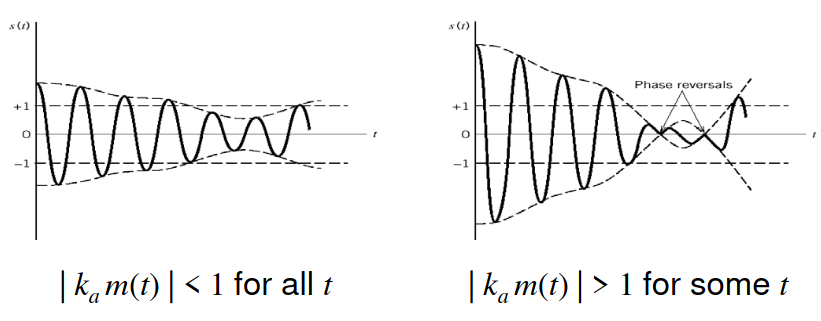
\includegraphics[width = 0.9\linewidth]{img/analog/AM/DSB.png}
    \caption{AM-DSB: onda modulada e sobremodulada, respetivamente.}
    \label{fig:DSB}
\end{figure}

%//==============================--@--==============================//%
\newpage
\subsubsection*{$\rightarrow$ Domínio da frequência}
\label{subsubsec:AM-freq-domain}

Recorrendo à transformada de Fourier, facilmente se obtém o espetro de $s(t)$:

$$
    \boxed{S(f) = \frac{A_c}{2}[\delta(f - f_c) + \delta(f + f_c)] + \frac{k_a A_c}{2}\left[M(f - f_c) + M(f + f_c)\right]}
$$

\noindent onde $M(f)$ é o espetro da mensagem e $M(f)\delta(f - f_c) = M(f - f_c)$, já que $\delta(f)$ é o elemento neutro da convolução.

\begin{figure}[H]
    \centering
    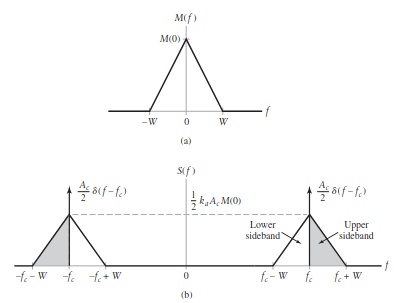
\includegraphics[width = 0.8\linewidth]{img/analog/AM/freqDomain.png}
    \caption{\textbf{(a)} Espetro da mensagem $m(t)$. \textbf{(b)} Espetro da onda modulada $s(t)$.}
    \label{fig:freqDomainDSB}
\end{figure}

\noindent $\pmb{\rightarrow}$ \textbf{\textit{Observações}}
\begin{itemize}
    \item[$\blacktriangle$] ``As a result of the modulation process, the spectrum of the message signal $m(t)$ for negative frequencies extending from $-W$ to 0 becomes completely visible for positive (i.e., measurable) frequencies, provided that the carrier frequency satisfies the condition $f_c >> W$.''\cite{Haykin2007}
    \item[$\blacktriangle$] ``For positive frequencies, the portion of the spectrum of an AM wave lying above the carrier frequency $f_c$ is referred to as the upper sideband, whereas the symmetric portion below $f_c$ is referred to as the lower sideband. The condition $f_c >> W$ ensures that the sidebands do not overlap.''\cite{Haykin2007} (Isto é, o envelope é visualizado).
    \item[$\blacktriangle$]``For positive frequencies, the highest frequency component of the AM wave equals $f_c + W$, and the lowest frequency component equals $f_c - W$. The difference between these two frequencies defines the transmission bandwidth $B_T = 2W$.\cite{Haykin2007}
\end{itemize}

%//==============================--@--==============================//%
\clearpage
\subsubsection[2.1.2 Detetor Envolvente]{$\rightarrow$ Detetor Envolvente}
\label{subsubsec:DetetorEnvolvente}

Admitindo que as \hyperref[subsubsec:AM-freq-domain]{condições supramencionadas} são garantidas, Para recuperar de novo o sinal $m(t)$ partindo da portadora modulada $x_{AM} (t)$ que chega ao recetor, basta rectificar a portadora e filtrar o resultado da rectificação por forma a preservar apenas as flutuações lentas do sinal retificado e que correspondem ao sinal $m(t)$, rejeitando as suas oscilações de alta frequência, usando para o efeito um filtro passa-baixo:

\begin{figure}[H]
    \centering
    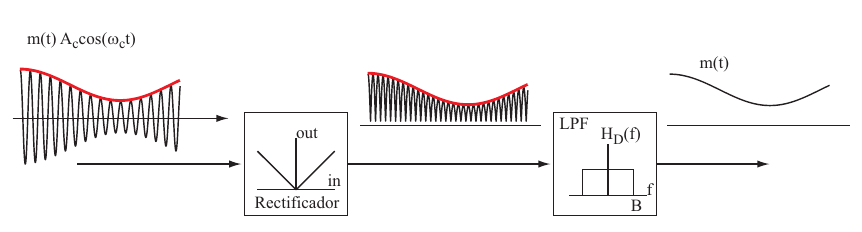
\includegraphics[width = 1\linewidth]{img/analog/AM/detetorEnvolvente.png}
    \caption{Diagrama Detetor Envolvente}
    \label{fig:DetetorEnvolvente}
\end{figure}

\noindent \textbf{$\rightarrow$ Nota}

\noindent A saída do retificador de onda completo é dada por:
$$
    y(t) = s(t) p(t)
$$
Onde $\boxed{p(t) = \text{sgn}[\cos{(2\pi f_c t)}]}$

\begin{figure}[H]
    \centering
    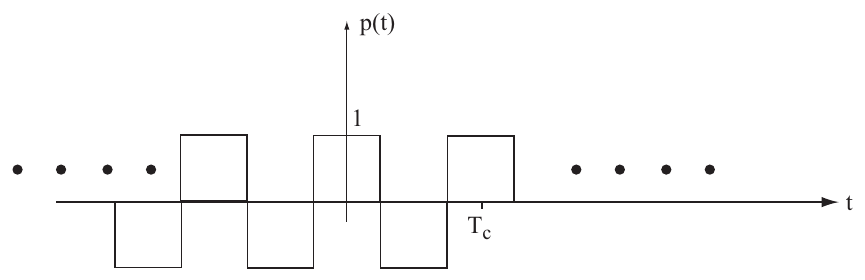
\includegraphics[width = 1\linewidth]{img/analog/AM/pt_envolvente.png}
    \caption{Sinal p(t).}
    \label{fig:p(t)}
\end{figure}

\noindent $p(t)$ é a extensão periódica de $\text{rect}\left(\dfrac{2t}{\text{T}_c}\right)$:

$$
    \boxed{P(f) = \mathcal{F}\{p(t)\} = \sum_{n=-\infty}^{\infty} \text{sinc}(2n)\delta(f - nf_0)}
$$

\noindent Consequentemente $y(t)$ possui uma réplica centrada em $f = 0$ que pode ser usada para recuperar integralmente o sinal $m(t)$ após filtragem pelo filtro de saída do detetor de envolvente.
\\\\
\noindent Por fim admite-se que à sa\'ida do receptor existe um condensador com a finalidade de remover a componente DC, $m_{dc}$ advinda do envelope, $[m_{dc} + k_a m(t)]$.

%//==============================--@--==============================//%
\subsubsection[2.1.3 Double Sideband Supressed Carrier]{$\rightarrow$ Double Sideband Supressed Carrier}
\label{subsubsec:DSB-SC}

``Basically, double sideband-suppressed carrier (DSB-SC) modulation consists of the product of the message signal $m(t)$ and the carrier wave $c(t)$, as shown in the equation:''\cite{Haykin2007}

$$
    \boxed{s(t) = c(t) m(t) = m(t) A_c \cos{(2\pi f_c t)}}
$$

\noindent Contrariamente à modulação anteriormente discutida, a modulação DSB-SC é anulada com o desaparecimento da mensagem de modulação. Neste sentido ``Transmitted power is saved here through the suppression of the carrier wave''\cite{Haykin2007} embora a largura de banda do canal se mantenha idêntica, nomeadamente $B_t = 2W$.
%//==============================--@--==============================//%
\subsubsection*{$\rightarrow$ Domínio da frequência}
\label{subsubsec:AM-freq-domain DSB-SC}

A transformada de Fourier de $s(t)$ é dada por

$$
    \boxed{S(f) = \frac{A_c}{2}\left[M(f - f_c) + M(f + f_c)\right]}
$$

\begin{figure}[H]
    \centering
    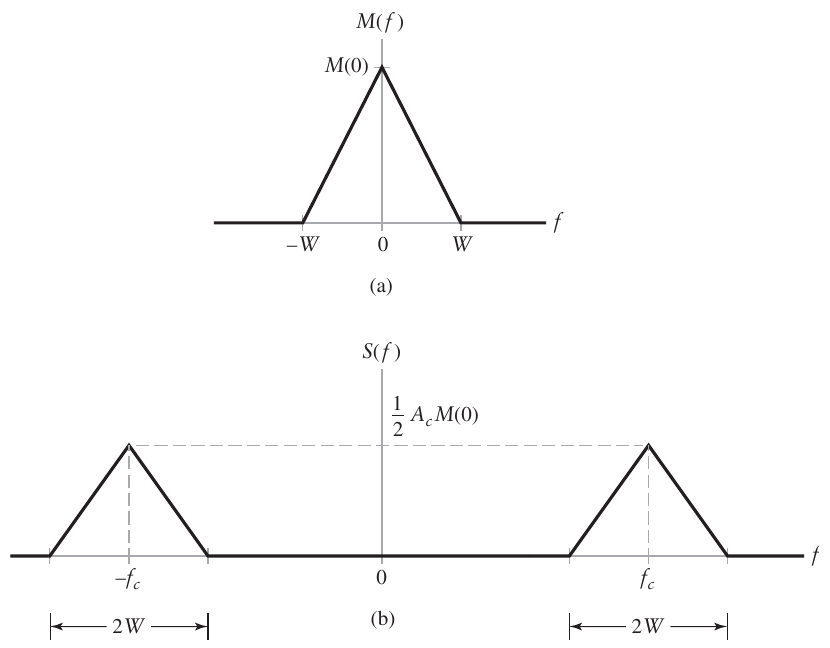
\includegraphics[width = 0.8\linewidth]{img/analog/AM/freqDomainDSB-DC.png}
    \caption{\textbf{(a)} Espetro da mensagem $m(t)$. \textbf{(b)} Espetro da onda modulada $s(t)$.}
    \label{fig:FreqDSB-DC}
\end{figure}

\noindent $\pmb{\rightarrow}$ \textbf{\textit{Observações}}
\begin{itemize}
    \item[$\blacktriangle$] ``Except for a change in scale factor, the modulation process simply translates the spectrum of the message signal by $f_c$ to the right and by $-f_c$ to the left. Of course, the transmission bandwidth required by DSB-SC modulation is the same as that for amplitude modulation namely, 2W.''\cite{Haykin2007}
\end{itemize}


%//==============================--@--==============================//%
\clearpage
\subsubsection[2.1.4 Detetor Coerente]{$\rightarrow$ Detetor Coerente}
\label{subsubsec:DetetorCoerente}
Se a amplitude do sinal modulante mudar de um valor positivo para um valor negativo, irá provocar inversões de fase na portadora modulada. Tal fenómeno é visível em casos de sobremodulação, inerentes à modulação DSB-SC, à qual o detetor envolvente é insensível. É então usado um desmodulador imune às inversões de fase, denominado detetor coerente ou síncrono:

\begin{figure}[H]
    \centering
    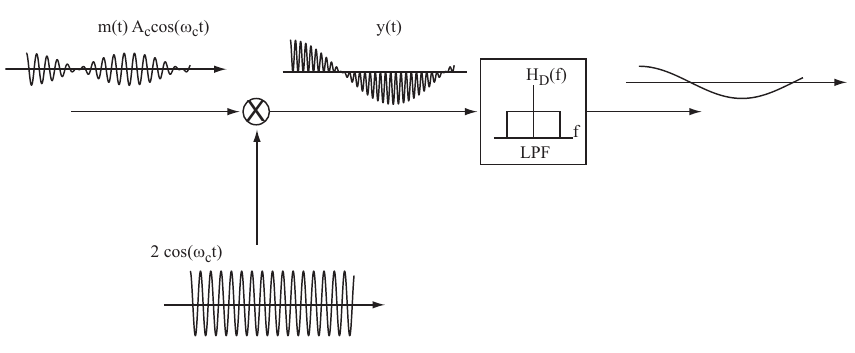
\includegraphics[width = 1\linewidth]{img/analog/AM/detetorSincrono.png}
    \caption{Diagrama do detetor coerente.}
    \label{fig:detetorCoerente}
\end{figure}

\noindent Avaliando o sinal à saída do modulador de produto (``assuming that the
local oscillator is out of phase by $f$ with respect to the sinusoidal carrier
 oscillator in the transmitter.''\cite{Haykin2007})

 $$
    y(t) = A'_c\cos{(2\pi f_c t + \Phi)}
 $$

%//==============================--@--==============================//%
\subsubsection[2.1.5 Potência de transmissão de uma onda modulada em amplitude]{$\rightarrow$ Potência de transmissão de uma onda modulada em amplitude}
\label{subsubsec:AM-power}

Tomando uma onda AM arbitrária da forma:
$$
    x_{\text{AM}}(t) = A_c[m_{dc} + m(t)] \cos(2\pi f_c t) 
$$
Verifica-se que a potência média do sinal, i.e., $<x_{\text{AM}}(t)>$ é dada por
$$
    P_T = \frac{A^2_c}{2}\left( m_{dc}^2 + P_m \right)
$$
em que $P_m$ é a potência média do sinal mensagem.

\paragraph[2.1.5.1 Eficiência de modulação de um sinal AM]{$\pmb{\star}$ Eficiência de modulação de um sinal AM}\mbox{}\\
 ``We define modulation efficiency as the ratio between the power of the part of the modulated signal that carries information about $m(t)$ and the total power of the modulated signal.''\cite{Nunes2015}
 $$
    \eta \delequal \frac{(A^2_c/2)P_m}{P_T} = \frac{P_m}{P_m + m_{dc}^2}
 $$
%//==============================--@--==============================//%
        %//==============================--@--==============================//%
\clearpage
\subsection{2.2 Modelação de Ângulo (PM e FM)}
\label{subsubsec:PM-FM}

Seja $\theta_i(t)$ o ângulo da portadora sinusoidal modulada que transporta o sinal mensagem. Exprime-se a resultante onde modulada como:
$$
    \boxed{ s(t) = A_c \cos\left[\theta_i(t)\right] }
    \quad \implies \quad
    f_i(t) = \frac{1}{2\pi} \frac{d \theta_i(t)}{dt}
$$

\begin{enumerate}
    \item[$\pmb{1.}$] \textit{Phase modulation} (PM): ``form of angle modulation in which the instantaneous angle $\theta_i(t)$ is varied linearly with the message signal $m(t)$''
    $$
        \pmb{\rightarrow} \theta_i(t) = 2\pi f_c t + k_p m(t)
    $$
    $$
        \therefore x_{\text{PM}}(t) = A_c \cos\left[ 2\pi f_c t + k_p m(t) \right]
    $$

    \item[$\pmb{2.}$] \textit{Frequency modulation} (FM): ``form of angle modulation in which the instanta- neous frequency $f_i(t)$ is varied linearly with the message signal $m(t)$''
    $$
        \pmb{\rightarrow} f_i(t) = f_c + f_\Delta\, m(t)
    $$
    $$
        \therefore x_{\text{FM}}(t) = A_c \cos\left[ 2\pi f_c t + 2\pi f_\Delta \int_{0}^{t} m(\tau) \, d\tau \right]
    $$
\end{enumerate}

\noindent em que $k_f$ representa o fator de \textit{phase-sensivity}, e $f_\Delta$ a \textit{frequency deviation}.
%//==============================--@--==============================//%
\subsubsection[2.2.1 Relação entre PM e FM]{$\rightarrow$ Relação entre PM e FM}
\label{subsubsec:PM-FM-relation}

Tendo em conta as definições acima, é natural verificar que um modulador de fase é realizável através de um modulador de frequência, e vice-versa.
%Adoro-te
\begin{figure}[H]
    \centering
    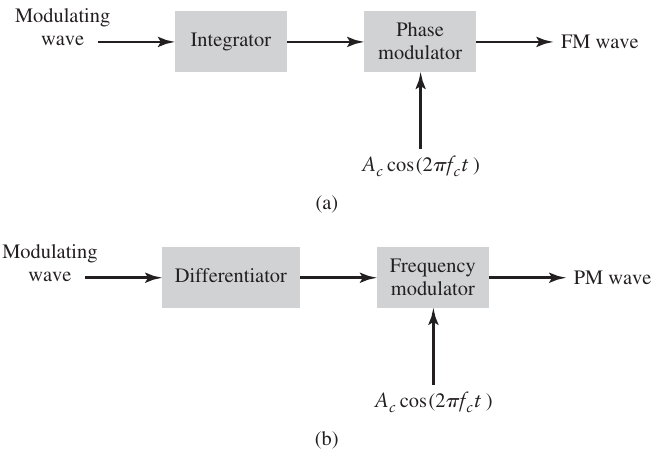
\includegraphics[width = 0.5\linewidth]{img/analog/FM/PM-FM-relation.png}
    \caption{``Illustration of the relationship between $[$FM$]$ and $[$PM$]$. (a) Scheme for generating an FM wave by using a phase modulator. (b) Scheme for generating a PM wave by using a frequency modulator.''\cite{Haykin2007}}
    \label{fig:PM-FM-relation}
\end{figure}

%//==============================--@--==============================//%
\subsubsection[2.2.2 Largura de banda FM (Carson's rule)]{$\rightarrow$ Largura de banda FM (Carson's rule)}
\label{subsubsec:FM}

\begin{theo}[\underline{Carson's rule} \cite{Haykin2007}]{def:carsons-rule}\label{def:carsons-rule}
$$
    B_T = 2(\beta + 1)W,\qquad \beta = \frac{f_\Delta\, \left[\text{max}\{m(t)\} - \text{min}\{m(t)\}\right]/2}{W}
$$
em que $\beta$ é o índice de modulação.
\end{theo}

\noindent ``The Carson’s rule shows that, for $\beta > 1$ (wideband FM), the bandwidth of the FM signals is much larger than that of the AM signals, for a given value of $W$.''\cite{Nunes2015}

\newpage

\iffalse
\noindent $\pmb{\rightarrow}$ \textbf{Nota:} ``The Carson’s rule provides sometimes a too small bandwidth estimate. A more approximated expression, for $\beta > 2$, would be $B_T = 2(\beta + 2)W$''\cite{Nunes2015}.
\fi

%//==============================--@--==============================//%
\paragraph[2.2.2.1 FM de banda estreita]{$\pmb{\star}$ FM de banda estreita (\textit{narrow-band})}\mbox{}\\
\noindent Supondo que $f_\Delta$ é tal que  
$$
    \left| 2\pi f_\Delta \int_{0}^{t} m(\tau)\, d\tau \right| \ll 1
$$
então
\begin{align*}
    x_{\text{FM}}(t) &= A_c \cos(2\pi f_c t) \cos( 2\pi f_\Delta \int_{0}^{t} m(\tau)\, d\tau ) - A_c \sin(2\pi f_c t) \sin( 2\pi f_\Delta \int_{0}^{t} m(\tau)\, d\tau ) \\
                     &\approx A_c \cos(2\pi f_c t) - A_c \sin(2\pi f_c t) \cdot \left( 2\pi f_\Delta \int_{0}^{t} m(\tau)\, d\tau \right)
\end{align*}
Isto indica que o sinal de banda estreita se aproxima de um sinal AM. Deste modo, a largura de banda será
$$
    B_T \approx 2B
$$
em que $B$ é a largura de banda do sinal fonte $m(t)$.

%//==============================--@--==============================//%
\paragraph[2.2.2.2 FM de banda larga]{$\pmb{\star}$ FM de banda larga (\textit{wide-band})}\mbox{}\\
Neste caso, temos que $f_\Delta \gg B$. A análise do sinal FM de banda larga é de natureza não trivial, pelo que se apresenta o ponto fulcral.
\\[6pt]
\noindent \textbf{Aproximação quasi-estacionária:} Caso $f_c \gg f_\Delta \gg B$, o espectro de potência do sinal FM é (aproximadamente) dado por:
$$
    S_x(f) = \frac{A^2}{4f_\Delta}\left[ f_x\left( -\frac{f+f_c}{f_\Delta} \right) + f_x\left( \frac{f-f_c}{f_\Delta} \right) \right]
$$
em que $f_x$ é a função de densidade de probabilidade.
\\[6pt]
\noindent Nestes moldes,
$$
     B_T \approx f_\Delta \cdot \left[ \text{max}\{m(t)\} - \text{min}\{m(t)\} \right]
$$
%//==============================--@--==============================//%
\subsubsection[2.2.3 Potência de transmissão de uma onda modulada em ângulo]{$\rightarrow$ Potência de transmissão de uma onda modulada em ângulo}
\label{subsubsec:FM-power}

Verifica-se que a amplitude de ondas PM e FM, $A_c$, se mantém constante ao longo do tempo, indepentemente do valor de $k_p$ ou de $f_\Delta$. Consequentemente, a potência média transmitida é uma contante dada por:
$$
    P_T = \frac{1}{2}A^2_c
$$
(é assumido que a resistência da carga é $1$ ohm).
%//==============================--@--==============================//%
\subsubsection[2.2.4 Discriminador de frequência (desmodulação de uma onda FM)]{$\rightarrow$ Discriminador de frequência (desmodulação de uma onda FM)}
\label{subsubsec:FM-discriminador}

\begin{figure}[H]
    \centering
    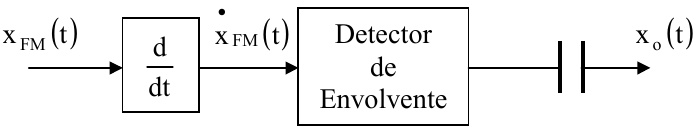
\includegraphics[width = 0.5\linewidth]{img/analog/FM/discriminadorFM.png}
    \caption{Discriminador de frequência\cite{Victor2010}.}
    \label{fig:FM-discriminador}
\end{figure}

$$
    \dot{x}_{FM}(t) = -2\pi A_c \left( f_c + f_\Delta m(t) \right) \sin(2\pi f_c t + 2\pi f_\Delta \int_{0}^{t} m(\tau)\, d\tau)
$$
 A saída do diferenciador não é mais do que uma portadora sinusoidal cuja envolvente vale $2\pi A_c (f_c + f_\Delta m(t))$, deste modo:
$$
    \because f_c \gg f_\Delta \implies x_0(t)\: \propto\: m(t)
$$
%//==============================--@--==============================//%

    \clearpage
    \section{3. Modelação Digital}
        %//==============================--@--==============================//%
\subsection[3.1 Amostragem (\textit{Sampling})]{$\rightarrow$ Amostragem (\textit{Sampling})}
\label{subsec:sampling}

Seja $x(t)$ um sinal arbitrário de energia finita. Supondo que o sinal é amostrado a uma cadência uniforme---a cada $T_S$ segundos---obtém-se, consequentemente, uma sequência de amostras espaçadas por este mesmo intervalo, $\{x(nT_S)\}$. Define-se $T_S$ $[$s$]$ como o período de amostragem, e $f_S \delequal 1/T_S$ como a frequência de amostragem $[$S/s$]$.

\vspace{0.75em}
\noindent Na sua forma geral, o processo resulta em:
$$
    \boxed{ x_s(t) = \sum_{n=-\infty}^{+\infty} x(nT_S)\, p(t-nT_S) }
$$
em que $p(t)$ é a forma do pulso utilizado. Na amostragem ideal, $p(t) \equiv \delta(t)$.

%//==============================--@--==============================//%
\subsubsection[3.1.1 Amostragem instantânea]{$\rightarrow$ Amostragem instantânea (\textit{instantaneous/ideal sampling})}
\label{subsubsec:instantaneous-sampling}
$$
    x_{\delta}(t) = \sum_{n=-\infty}^{+\infty} x(nT_S)\, \delta(t-nT_S) \,\xleftrightharpoons[\mathcal{F}]{}\, X_{\delta}(f) = f_S \sum_{m=-\infty}^{+\infty} X(f-m f_S)
$$

\vspace{-1em}
\begin{theo}[\underline{Teorema da Amostragem} (Teorema de Nyquist-Shannon)]{teo:sampling}\label{teo:sampling}
    Seja $x(t)$ um sinal de energia finita (banda limitada), com frequências não superiores a $W$. Então, este sinal é totalmente descrito através de uma coleção de amostras espaçadas por $1/(2W)$ segundos; sendo perfeitamente reconstruído através destas amostras.

    \vspace{0.5em}
    \noindent A \underline{menor frequência} de amostragem possível que não resulta em \textit{aliasing} é
    $$
        f_S = f_N \delequal 2W
    $$
    denominada por \underline{frequência de Nyquist}. $\pmb{\rightarrow}$ \textbf{Critério de Nyquist:} $f_S \geq f_N$ 

    \vspace{0.75em}
    \noindent \textbf{Nota:} Por vezes é definida uma banda de guarda, e deste modo: $f_S \delequal f_{S0} + B_G$
\end{theo}

\begin{figure}[H]
    \centering
    \begin{minipage}[c]{0.5\textwidth}
        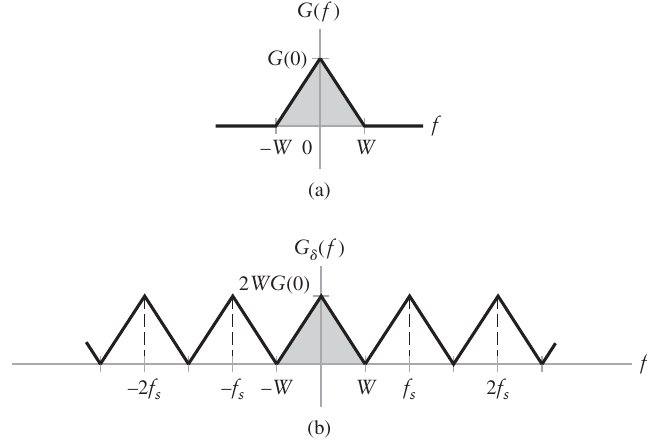
\includegraphics[width = 1\linewidth]{img/digital/sampling/sampling-frequency-domain.png}
    \end{minipage}
    \raisebox{0em}{
    \hspace*{0.5em}\begin{minipage}[c]{0.4\textwidth}
        \caption{(a) Espectro do sinal de banda limitada $g(t)$. (b) Espectro da versão amostrada idealmente, $g_\delta(t)$, a um ritmo de $T_S = 1/(2W)$ (não ocorre \textit{aliasing}).}
        \label{fig:sampling-frequency-domain}
        
        \vspace{-1.5em}
        \begin{theo}[\underline{\textit{Aliasing}}]{def:aliasing}\label{def:aliasing}
            Se o critério de Nyquist não se verificar satisfeito, as cópias adjacentes sobrepõem-se e não é possível discernir um $X(f)$ não ambíguo.
        \end{theo}       
    \end{minipage}}
\end{figure}

\renewcommand*{\thefootnote}{\fnsymbol{footnote}}
\footnotetext[4]{%
    Tomando uma $f_S = 2W$, e assumindo um filtro passa-baixo ideal para a reconstrução do sinal com uma frequência de corte $f_c = f_S/2 = W$, obtém-se a expressão:
    $$
        x(t) = \sum_{n=-\infty}^{+\infty} x\left(\frac{1}{2W}\right)\, \text{sinc}(2W t - n),\quad -\infty < t < +\infty
    $$
    denominada por \textit{interpolation formula}---para reconstruir o sinal $x(t)$ através de uma sequência de valores amostrados $\{x(nT_S)\}$, em que a função sinc($2W t - n$) é a \textit{interpolation function}.
}
\renewcommand*{\thefootnote}{\arabic{footnote}}
%adoro-te :3
%//==============================--@--==============================//%
        \clearpage
%//==============================--@--==============================//%
\subsection[3.2 Pulse Amplitude Modulation]{3.2 Pulse Amplitude Modulation}
\label{subsec:PAM}


%//==============================--@--==============================//%
        \clearpage
%//==============================--@--==============================//%
\subsection[3.3 Pulse Code Modulation]{$\rightarrow$ Pulse Code Modulation}
\label{subsec:PCM}

\begin{theo}[\underline{Pulse Code Modulation (PCM)} \cite{Haykin2007}]{teo/def:PCM}\label{teo/def:PCM}
     ``In pulse-code modulation (PCM), a message signal is represented by a sequence of coded pulses, which is accomplished by representing the signal in discrete form in both time and amplitude.''
\end{theo}

%//==============================--@--==============================//%
\subsubsection[3.3.1 Quantização]{}
\label{subsubsec:quantization}
\vspace{-3em}
\begin{theo}[\underline{Quantização} \cite{Haykin2007}]{teo/def:Quantization}\label{teo/def:Quantization}
 ``Amplitude quantization is defined as the process of transforming the sample amplitude $m(nT_s)$ of a baseband signal $m(t)$ at time $t = nT_s$ into a discrete amplitude $v(nT_s)$ taken from a finite set of possible levels.''
\end{theo}
%//==============================--@--==============================//%
\vspace{-2em}
\paragraph[3.3.1.1 Quantização Uniforme]{$\pmb{\star}$ Quantização Uniforme:}
Todos os intervalos possuem comprimentos idênticos $\Delta$.
\label{subsubsec:quantizationU}
\vspace{-1em}
\begin{figure}[H]
    \centering
    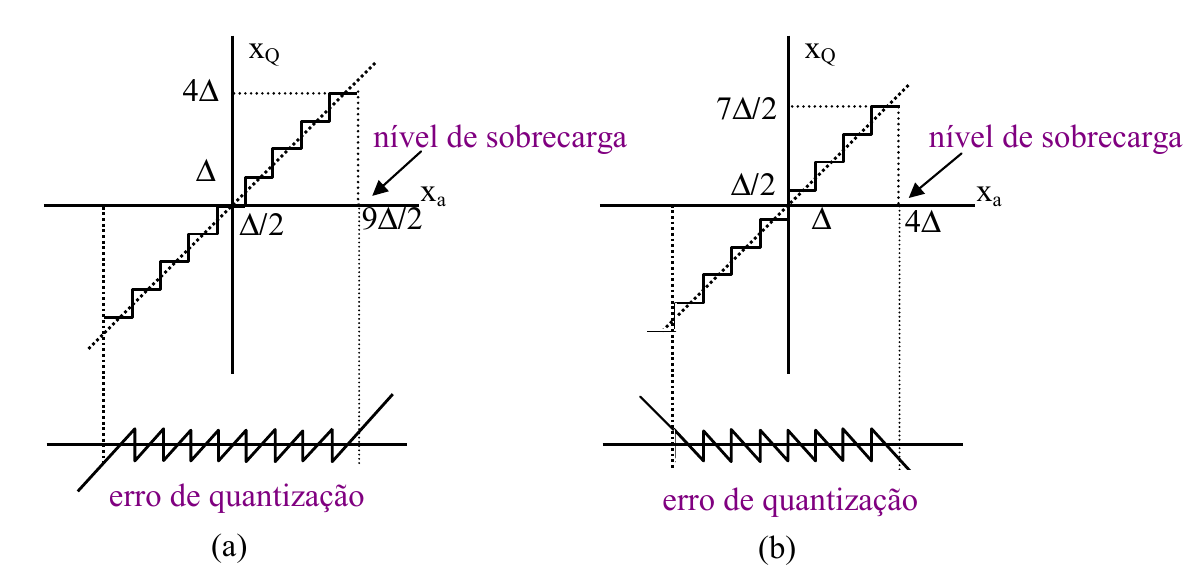
\includegraphics[width = 0.8\linewidth]{img/digital/PCM/QuantizacaoU.png}
    \caption{Características e erro de quantização uniforme: (a) ímpar; (b) par}
    \label{fig:QuantizacaoU}
\end{figure}

\noindent Os dois tipos de característica de quantização ilustradas na \hyperref[fig:QuantizacaoU]{Fig. 7} diferem apenas na forma como cruzam a origem, Formando um número ímpar (\textit{midtread}) ou par (\textit{midrise}) de níveis de quantização (de entrada, $x_a$). Inversamente o passo $\Delta$ dos intervalos de saída, $x_Q$ é par (a) e ímpar (b).
\\
\noindent O número de níveis de quantização em utilização é definido por:
$$
    \boxed{M = \frac{\left|\text{Range}\right|}{\Delta}}
$$
Onde o Range denota o intervalo de amplitudes que o sinal analógico pode tomar. 
\\\\
Subsequentemente, cada um dos $M$ níveis de quantização é codificado por uma palavra de comprimento $L$ onde:
$$
    \boxed{M = n^\text{L}}
$$
Onde $n$ está dependente do sistema PCM em uso (binário: $n = 2$, trenário $n = 3$, quaternário: $n = 4$, ...).

\noindent A geração destas palavras de comprimento $L$ $[$símbolos/sample$]$ não poderá exceder a duração do período de amostragem. É então definido a taxa de geração de dados:
$$
    \boxed{r_s \ge f_s \text{L} \quad [\text{Baud}]}
$$

\noindent onde $f_s$ é a frequência de amostragem e Baud denota a taxa de transmissão de símbolos por segundo.
%adoro-te cutie :3 adoro-te 
%//==============================--@--==============================//%
\paragraph[3.3.1.2 Relação Sinal–Ruído de Quantização]{$\pmb{\star}$ Relação Sinal–Ruído de Quantização}
\mbox{}\\
O erro de quantização definido pela variável aleatória:
$$
    \text{e}(\text{kT}_a) = x_Q(\text{kT}_a) - x_a(\text{kT}_a)
$$
Denomina a diferença entre as amplitudes de entrada e os passos da saída. Tal erro tomará valores que em módulo podem ser muito elevados. De uma forma geral, a discretização das amplitudes de entrada deve ser grande o suficiente de forma a que o o módulo do erro seja sempre inferior a metade do passo:

$$
    \boxed{|\text{e}(\text{kT}_a)| \le \frac{\Delta}{2}}
$$
Para quantificar o desempenho do processo de digitalização–reconstrução usa-se com o medida a relação sinal – ruído de quantização aqui designada por SQNR:
$$
    \boxed{\text{SQNR} = \frac{\text{P}_x}{\text{P}_e}}
$$
em que $P_x$ é a potência do sinal amostrado $x_a(t)$. Para variáveis aleatórias a potência do sinal, é dada por:
$$
    \boxed{P_x = R_x(0) = \text{E}\{x_a(t)^2\} = \int_{-\infty }^{\infty}x^2f(x)\, dx}
$$
onde $f(x)$ é a função de densidade de probabilidade de amplitude.

\vspace{0.5em}
\noindent $P_e$ é a potência do erro, que pode ser aproximado a:
$$
    \boxed{P_e \approx \frac{\Delta^{2}}{12}} 
$$

\noindent É trivialmente concluido que a SQNR diminui quando o comprimento do intervalo de quantização aumenta, o que se traduz numa reconstrução menos precisa do sinal original.

%//==============================--@--==============================//%
\paragraph[3.3.1.3 Quantização Não Uniforme]{$\pmb{\star}$ Quantização Não Uniforme:}
\label{subsubsec:quantizationNU}
A quantização não uniforme visa usar intervalos de quantização mais longos para
amostras que ocorrem em intervalos de menor probabilidade e intervalos de quantização de
menor comprimento no caso contrário. A escolha destes comprimentos deverá portanto ser
feita por forma a otimizar, o desempenho do processo de digitalização–reconstrução.

\vspace{0.5em}
\noindent Esta compressão de intervalos é realizada com base na lei de $\mu$ ou a lei de $A$ (europeia):
\begin{align*}
    |v_\mu| &= \frac{\ln(1 + \mu|m/m_p|)}{\ln(1+\mu)}\text{sgn}(m) &(\mu\textit{-law})\\[6pt]
    |v_A| &= \begin{cases} 
        \dfrac{A |m|}{1 + \ln A}, & |m| \in [0, 1/A] \\[16pt]
        \dfrac{1+\ln(A|m|)}{1+\ln A}, & |m| \in [1/A, 1]
    \end{cases} &(A\textit{-law})
\end{align*}
em que $|m|$ é o \textit{input} normalizado e $|v|$ a saída normalizada.

%//==============================--@--==============================//%
\clearpage
\subsubsection[3.3.2 Gerador de Sinais PCM]{$\rightarrow$ Gerador de Sinais PCM}
\label{subsubsec:arquiteturaPCM}

\begin{figure}[H]
    \centering
    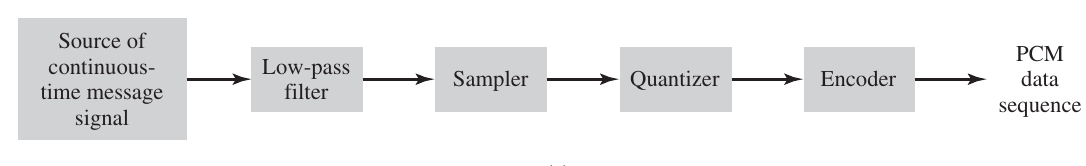
\includegraphics[width = 1\linewidth]{img/digital/PCM/PCM_ARQ.png}
    \caption{Arquitectura do Sistema Gerador de Sinais PCM}
    \label{fig:PCM_ARQ}
\end{figure}

\begin{enumerate}
    \item \textbf{Sampling (amostragem):} O sinal analógico (\textit{continuous-time message signal}) é amostrado com recurso a um pente de pulsos retangulares (\textit{sample and hold}), garantindo um ritmo de amostragem superior ao dobro da componente de frequência mais elevada da mensagem, 2W. (Na prática é utilizado um filtro \textit{antialiasing} ``in order to exclude frequencies greater than W before sampling''\cite{Haykin2007}).
    
    \item \textbf{Quantization (Quantização):} O sinal amostrado é quantizado, tornando-se discreto no tempo e na amplitude (\textit{vide} \hyperref[subsubsec:quantization]{secção sobre a quantização}).
    
    \item \textbf{Encoding:} Posteriormente, o sinal discretizado sofre um ``encoding process to translate the discrete set of sample values to a more appropriate form of signal. Any plan for representing this discrete set of values as a particular arrangement of discrete events is called a code.''\cite{Haykin2007}
\end{enumerate}

\paragraph[3.3.2.1 Line Codes]{$\pmb{\star}$ Line Codes (Códigos de sinalização binária)}
\begin{theo}[\underline{Line Codes} \cite{Haykin2007}]{teo/def:Line Codes}\label{teo/def:LineCodes}
 ``In reality, PCM (...) represent different strategies for source encoding, whereby
an analog signal is converted into digital form. However, all three of them share a common
feature: once a binary sequence of 1s and 0s is produced, a line code is needed for electrical representation of that binary sequence.''
\end{theo}

\noindent De uma forma geral, um código de linha pode ser representado por:
$$
    s(t) = \sum_{n=-\infty}^{\infty} a_n g(t - nT_b)
$$

\noindent Onde $g(t)$ denota a forma do impulso $n$, $a_n$ a sua magnitude e $T_b$ a duração do bit. 

\noindent De uma forma geral, podemos definir o espetro de potência de um código de linha como:
$$
    \boxed{S_s(f) = \frac{|G(f)|^2}{T_b}\sum_{k = -\infty}^{\infty}R(k)e^{j2\pi f k T_b}}\qquad
    \boxed{R(k) = \sum_{i = 1}^{I} a_{n}a_{n+k}p_i}
$$

\noindent Onde $R(0)$ corresponde à potência da sinalização e a largura de banda é definida pelo intervalo de frequências que contem a maior parte da energia do sinal:

$$
    \boxed{B_T = f_T - 0}
$$%miminhos :3 cutie

%//==============================--@--==============================//%
\clearpage
\paragraph*{Unipolar NRZ\protect\footnotemark[2]}\mbox{}\\
\label{line:unipolarNRZ}
\begin{figure}[H]
    \centering
    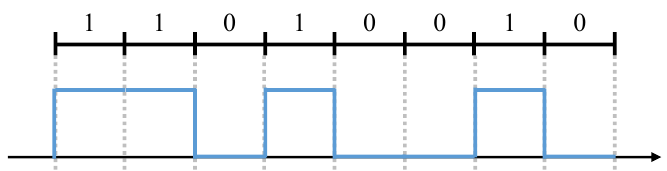
\includegraphics[width = 0.8\linewidth]{img/digital/line-codes/LUnipolarNRZ.png}
    \caption{Unipolar NRZ (11010010).}
    \label{fig:LUnipolarNRZ}
\end{figure}
\noindent Um código unipolar NRZ possui pulsos do tipo:
$$
    g(t) = \text{rect}\left(\frac{t}{T_b}\right)
$$
\noindent Com o respetivo espetro de potência:

$$
    \boxed{S_s(f) = \frac{A^2 T_b}{4}\, \text{sinc}(fT_b)^2\left[1 + \frac{1}{T_b}\delta(f)\right]}
$$

\noindent E potência e largura de banda (supondo que o sinal atinge a grande maioria da sua energia após o primeiro zero do espetro de potência):
%adoro-te
\begin{figure}[H]
    \centering
    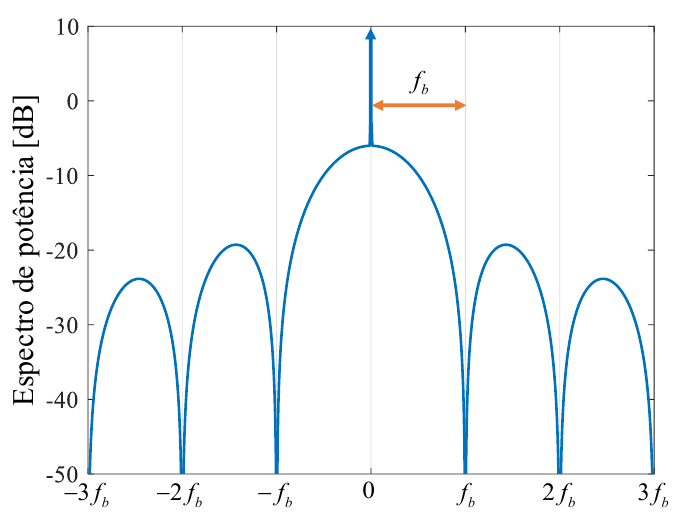
\includegraphics[width = 0.7\linewidth]{img/digital/line-codes/PUnipolarNRZ.png}
    \caption{Espetro de Potência unipolar NRZ.}
    \label{fig:PUnipolarNRZ}
\end{figure}

$$
    \boxed{P = R(0) = A^2}\qquad
    \boxed{B_T = f_{\text{1º zero}} - 0 = \frac{1}{T_b}}
$$

\footnotetext[2]{A vizualização dos códigos de sinalização binária subsequente no domínio do tempo será realizada mediante o código 11010010.}

%//==============================--@--==============================//%
\clearpage
\paragraph*{Unipolar RZ}\mbox{}\\
\label{line:unipolarRZ}
\begin{figure}[H]
    \centering
    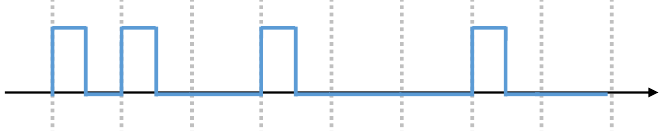
\includegraphics[width = 0.8\linewidth]{img/digital/line-codes/LUnipolarRZ.png}
    \caption{Unipolar NRZ (11010010).}
    \label{fig:LUnipolarRZ}
\end{figure}
\noindent Um código unipolar RZ (com um \textit{duty-cycle} de $50\%$) possui pulsos do tipo:
$$
    g(t) = \text{rect}\left(\frac{2t}{T_b}\right)
$$
\noindent Com o respetivo espetro de potência:

$$
    \boxed{S_s(f) = \frac{A^2 T_b}{16}\, \text{sinc}(fT_b/2)^2\left[1 + \frac{1}{T_b}\sum_{k = -\infty}^{k = \infty}\delta(f-kT_b/2)\right]}
$$

\noindent E potência e largura de banda (supondo que o sinal atinge a grande maioria da sua energia após o primeiro zero do espetro de potência):

\begin{figure}[H]
    \centering
    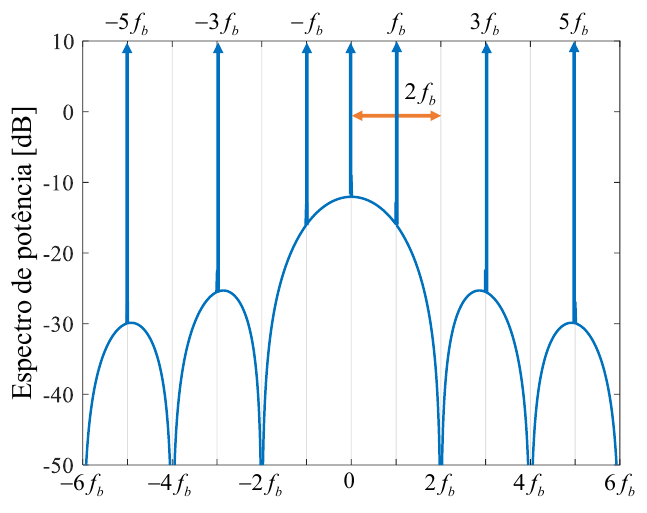
\includegraphics[width = 0.7\linewidth]{img/digital/line-codes/PUnipolarRZ.png}
    \caption{Espetro de Potência unipolar RZ.}
    \label{fig:PUnipolarRZ}
\end{figure}

$$
    \boxed{P = R(0) = \frac{A^2}{4}}\qquad
    \boxed{B_T = f_{\text{1º zero}} - 0 = \frac{2}{T_b}}
$$

\noindent A potência média deste código será de metade do código Unipolar NRZ, uma vez que, é emitida a mesma energia, nos símbolos com amplitude maior que zero, mas em metade do tempo.
%//==============================--@--==============================//%
\clearpage
\paragraph*{Polar NRZ}\mbox{}\\
\label{line:polarNRZ}
\begin{figure}[H]
    \centering
    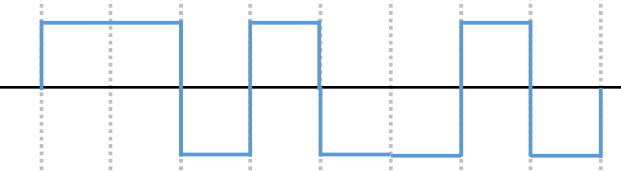
\includegraphics[width = 0.8\linewidth]{img/digital/line-codes/LPolarNRZ.png}
    \caption{Polar NRZ (11010010).}
    \label{fig:polarNRZ}
\end{figure}
\noindent Um código Polar NRZ possui pulsos do tipo:
$$
    g(t) = \text{rect}\left(\frac{t}{T_b}\right)
$$
\noindent Com o respetivo espetro de potência:

$$
    \boxed{S_s(f) = A^2 T_b\, \text{sinc}(fT_b)^2}
$$

\noindent E potência e largura de banda (supondo que o sinal atinge a grande maioria da sua energia após o primeiro zero do espetro de potência):

\begin{figure}[H]
    \centering
    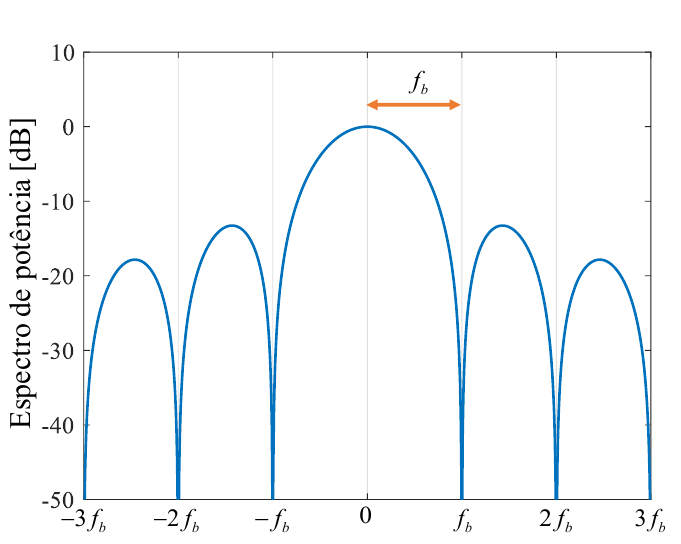
\includegraphics[width = 0.7\linewidth]{img/digital/line-codes/PPolarNRZ.png}
    \caption{Espetro de Potência polar NRZ.}
    \label{fig:PpolarNRZ}
\end{figure}

$$
    \boxed{P = R(0) = A^2}\qquad
    \boxed{B_T = f_{\text{1º zero}} - 0 = \frac{1}{T_b}}
$$
%//==============================--@--==============================//%
\clearpage
\paragraph*{Polar RZ}\mbox{}\\
\label{line:polarRZ}
\begin{figure}[H]
    \centering
    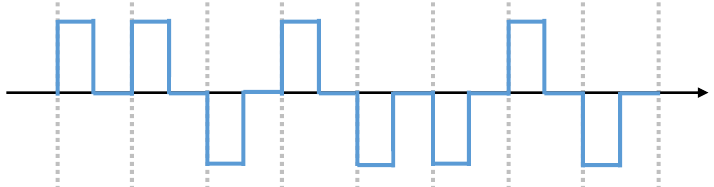
\includegraphics[width = 0.8\linewidth]{img/digital/line-codes/LPolarRZ.png}
    \caption{Polar RZ (11010010).}
    \label{fig:LPolarRZ}
\end{figure}
\noindent Um código Polar RZ (com um \textit{duty-cycle} de $50\%$) possui pulsos do tipo:
$$
    g(t) = \text{rect}\left(\frac{t}{2T_b}\right)
$$
\noindent Com o respetivo espetro de potência:

$$
    \boxed{S_s(f) = \frac{A^2 T_b}{4}\, \text{sinc}(fT_b)^2}
$$

\noindent E potência e largura de banda (supondo que o sinal atinge a grande maioria da sua energia após o primeiro zero do espetro de potência):

\begin{figure}[H]
    \centering
    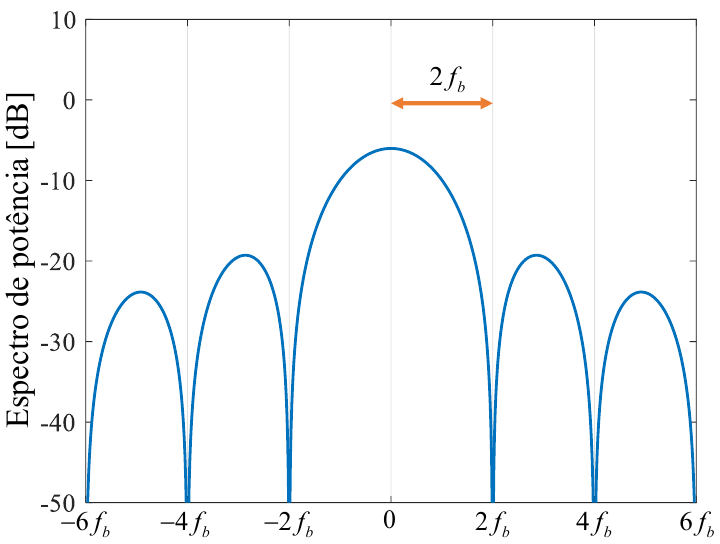
\includegraphics[width = 0.7\linewidth]{img/digital/line-codes/PPolarRZ.png}
    \caption{Espetro de Potência: Polar RZ.}
    \label{fig:PPolarRZ}
\end{figure}

$$
    \boxed{P = R(0) = \frac{A^2}{2}}\qquad
    \boxed{B_T = f_{\text{1º zero}} - 0 = \frac{2}{T_b}}
$$

%//==============================--@--==============================//%
\clearpage
\paragraph*{Bipolar NRZ}\mbox{}\\
\label{line:bipolarNRZ}
\begin{figure}[H]
    \centering
    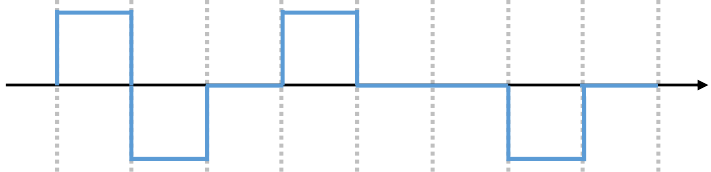
\includegraphics[width = 0.8\linewidth]{img/digital/line-codes/LBipolarNRZ.png}
    \caption{Bipolar NRZ (11010010).}
    \label{fig:bipolarNRZ}
\end{figure}
\noindent Um código Bipolar NRZ possui pulsos do tipo:
$$
    g(t) = \text{rect}\left(\frac{t}{T_b}\right)
$$
\noindent Com o respetivo espetro de potência:

$$
    \boxed{ S_s(f) = \frac{A^2 T_b}{2} \left[\text{sinc}(f T_b)\right]^2 \cdot \left[\sin(\pi f T_b)\right]^2 }
$$

\noindent E potência e largura de banda (supondo que o sinal atinge a grande maioria da sua energia após o primeiro zero do espetro de potência):

\begin{figure}[H]
    \centering
    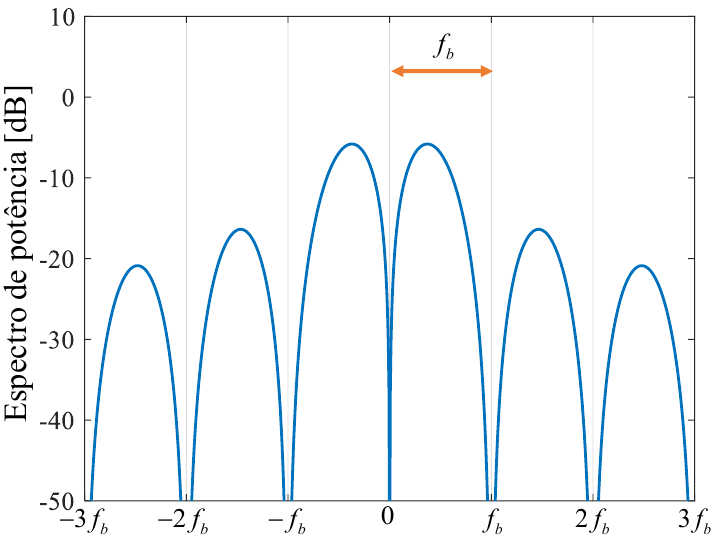
\includegraphics[width = 0.7\linewidth]{img/digital/line-codes/PBipolarNRZ.png}
    \caption{Espetro de Potência: Bipolar NRZ.}
    \label{fig:PBipolarNRZ}
\end{figure}

$$
    \boxed{P = R(0) = \frac{A^2}{2}}\qquad
    \boxed{B_T = f_{\text{1º zero}} - 0 = \frac{1}{T_b}}
$$

%//==============================--@--==============================//%
\clearpage
\paragraph*{Bipolar RZ}\mbox{}\\
\label{line:bipolarRZ}
\begin{figure}[H]
    \centering
    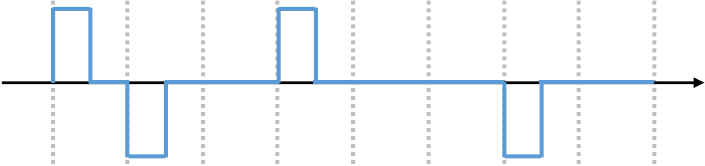
\includegraphics[width = 0.8\linewidth]{img/digital/line-codes/LBipolarRZ.png}
    \caption{Bipolar RZ (11010010).}
    \label{fig:bipolarRZ}
\end{figure}
\noindent Um código Bipolar RZ (com um \textit{duty-cycle} de $50\%$) possui pulsos do tipo:
$$
    g(t) = \text{rect}\left(\frac{t}{2T_b}\right)
$$
\noindent Com o respetivo espetro de potência:

$$
    \boxed{ S_s(f) = \frac{A^2 T_b}{8}\, \left[\text{sinc}(f\frac{T_b}{2})\right]^2 \cdot \left[\sin(\pi f \frac{T_b}{2})\right]^2 }
$$

\noindent E potência e largura de banda (supondo que o sinal atinge a grande maioria da sua energia após o primeiro zero do espetro de potência):

\begin{figure}[H]
    \centering
    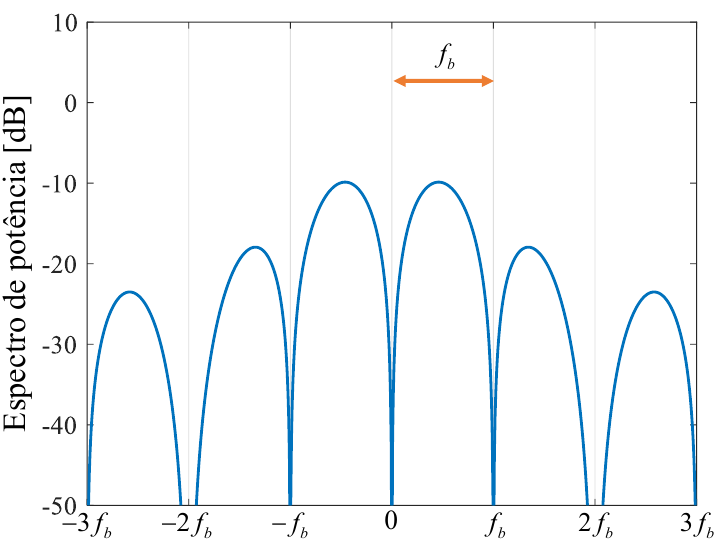
\includegraphics[width = 0.7\linewidth]{img/digital/line-codes/PBipolarRZ.png}
    \caption{Espetro de Potência polar NRZ.}
    \label{fig:PBipolarRZ}
\end{figure}

$$
    \boxed{P = R(0) = \frac{A^2}{4}}\qquad
    \boxed{B_T = f_{\text{1º zero}} - 0 = \frac{1}{T_b}}
$$

%//==============================--@--==============================//%
\clearpage
\paragraph*{Manchester}\mbox{}\\
\label{line:manchester}
\begin{figure}[H]
    \centering
    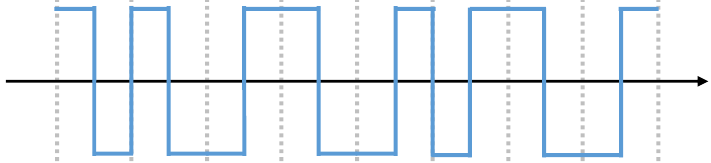
\includegraphics[width = 0.8\linewidth]{img/digital/line-codes/LManchester.png}
    \caption{Manchester (11010010).}
    \label{fig:manchester}
\end{figure}
\noindent Um código Manchester possui pulsos do tipo:
$$
    g(t) = \text{rect}\left(\frac{t+T_b/4}{2T_b}\right) - \text{rect}\left(\frac{t - T_b/4}{2T_b}\right) 
$$
\noindent Com o respetivo espetro de potência:

$$
    \boxed{S_s(f) = A^2 T_b\, \left[\text{sinc}(f\frac{T_b}{2})\right]^2 \cdot \left[\sin(\pi f \frac{T_b}{2})\right]^2 }
$$

\noindent E potência e largura de banda (supondo que o sinal atinge a grande maioria da sua energia após o primeiro zero do espetro de potência):

\begin{figure}[H]
    \centering
    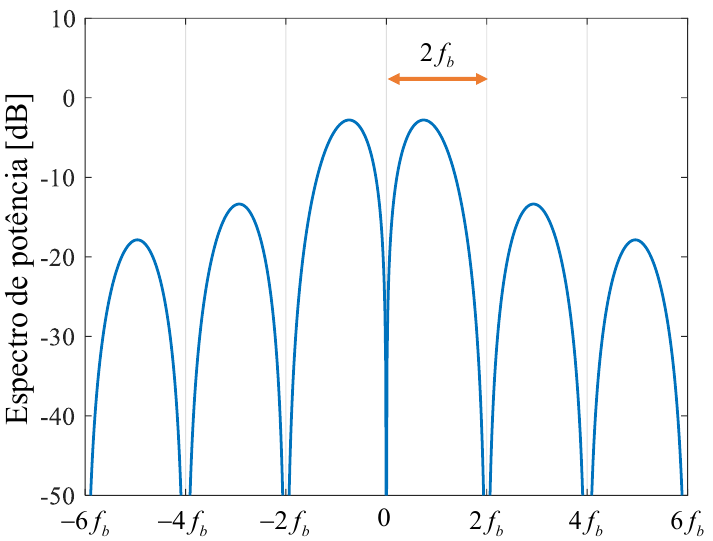
\includegraphics[width = 0.7\linewidth]{img/digital/line-codes/PManchester.png}
    \caption{Espetro de Potência: Manchester.}
    \label{fig:PManchester}
\end{figure}

$$
    \boxed{P = R(0) = A^2}\qquad
    \boxed{B_T = f_{\text{1º zero}} - 0 = \frac{2}{T_b}}
$$
%//==============================--@--==============================//%
        %//==============================--@--==============================//%
\clearpage
\subsection[3.4 Interferência intersimbólica]{$\rightarrow$ Interferência intersimbólica}
\label{subsec:intersymbol-interference}

\begin{figure}[H]
    \centering
    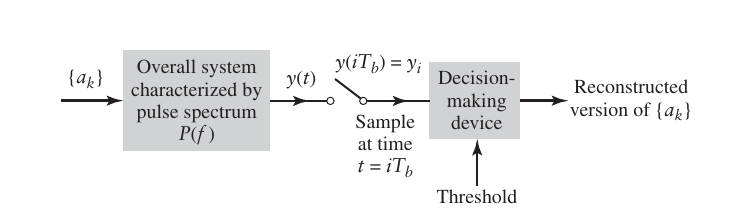
\includegraphics[width = 0.8\linewidth]{img/digital/ISI/Receiver.png}
    \caption{Sistema de receção simplificado.}
    \label{fig:recetor}
\end{figure}

À entrada do \textit{sampler} do esquema do sistema de receção simplificado encontra-se um sinal PAM com pulso $p(t)$ e coeficientes $a_k$ (onde $a_0 = -1$ codifica o bit 0 e $a_1 = +1$ codifica o bit 1):

$$
    x(t) = \sum_{n = -\infty}^{\infty}p(t - n T_b)
$$

\noindent O sinal é amostrado sincronamente com o transmissor:
$$
    x(i T_b) = \sum_{n = -\infty}^p((i - n)T_b)
$$

\noindent Para $n = i$, $p(0) = \sqrt{E}$ (\textit{transmitted signal energy per bit (symbol)}). Onde $n = i$ traduz a sincronia entre i, o instante em que o sinal é amostrado no recetor e n, simbolo do \textit{data stream} produzido pelo transmissor. Isolando o termo para o qual $n = i$ obtemos:

$$
    \boxed{x(i T_b) = a_i\sqrt{E} + \sum_{\substack{n = -\infty\\
                                        n \neq i}}^p((i - n)T_b)}
$$

\noindent A decodificação do símbolo $i$ onde $x_i = \sqrt{E}a_i$ (\textit{perfect decoding}, $a_i$ representa o símbolo binário, com a exceção de um fator multiplicativo) é acompanhada de ruído residual denotado por interferência intersimbólica. A arquitetura do recetor deve ser robusta o suficiente de forma a mitigar/eliminar o ruído adicional.

%//==============================--@--==============================//%
\subsubsection[3.4.1 Critério de Nyquist]{$\rightarrow$ Nyquist Channel}
\label{subsec:NyqCriterion}
O pulso ideal que garante a mitigação da IIS na entrada do \textit{sampler} satisfaz as seguintes duas condições:
$$
    p(t) = \begin{cases}
        1 & t = 0\\
        0 & t \neq 0\\
    \end{cases}
$$

\noindent Amostrando o pulso nos instantes de T: 
$$
    p\delta(t) = \sum_{k = -\infty}^{\infty}p(kT)\delta(t - kT)
$$
\noindent subsequentemente, recorrendo à sua transformanda:
$$
    P\delta(f) = \frac{1}{T}\sum_{k = -\infty}^{\infty}P(f - k/T) = \sum_{k = -\infty}^{\infty}P(kT)e^{-2\pi f T} = p(0) = 1
$$
\clearpage
\noindent Logo podemos admitir que:

$$
    \boxed{P_\delta(f) = \sum_{k = -\infty}^{\infty}P(f - rk) = T}
$$

\noindent Para que que a soma ponto a ponto em $f$ de todas as versões de $P(f)$ transladadas seja constante, garantindo a diminuição de ruído residual é necessário que:

$$
    \boxed{r = 2B_0}
$$

\noindent Onde $B_0$ é a largura de banda fundamental do sinal (\textit{vide} \hyperref[line:unipolarNRZ]{secção sobre \textit{line codes}}, é a largura que alberga a grande maioria da energia do sinal). Supondo um pulso retangular a condição é garantida:

\begin{figure}[H]
    \centering
    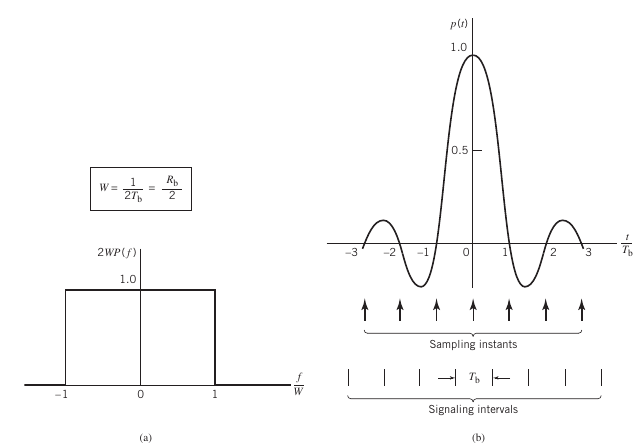
\includegraphics[width = 1\linewidth]{img/digital/ISI/Nyq.png}
    \caption{ (a) Resposta ideal em magnitude. (b) Pulso ideal.}
    \label{fig:Nyq}
\end{figure}

\mdfsetup{linewidth=2pt}
\begin{mdframed}
$\pmb{\star}$ \textbf{Nota:}
\mbox{}\\
Esta relação garante-se apenas para códigos do tipo NRZ, para códigos RZ o pulso dura metade do tempo de bit (símbolo), $r = 2/T$ logo a relação altera-se:
$$
    \boxed{r = B_0}
$$
\noindent Ainda, para um sistema de N níveis (sistemas quaternários, trenários \dots) o \textit{rate} de símbolo relaciona-se com o \textit{rate} de bit da seguinte forma:
$$
\boxed{r_b = \log_2 (M) r_s}
$$
\end{mdframed}
%//==============================--@--==============================//%
\clearpage
\subsubsection[3.4.2 Espetro Raised Cosine]{$\rightarrow$ Espetro Raised Cosine}
\label{subsec:RRC}

``To ensure physical realizability of the overall pulse spectrum $P(f)$, we need a solution that differs from the Nyquist channel in one important respect: the modified $P(f)$ decreases toward zero gradually rather than abruptly. In more specific terms, P1f2 is proposed to consist of two portions:
\begin{enumerate}
    \item Flat portion, which occupies the frequency band $0 \leq |f| \leq f_1$ for some parameter $f_1$ to be defined.
    \item Roll-off portion, which occupies the frequency band $f_1 < |f| < 2B_0  f_1$
\end{enumerate}
For obvious reasons, the $P(f)$ constructed in this manner is called the raised cosine pulse spectrum.''\cite{Haykin2007}
$$
    P(f) = \begin{cases}
            \dfrac{1}{2B_0} & 0 \leq |f| < f_1\\
            \dfrac{1}{4B_0}\left\{1 + \cos(\left[\dfrac{\pi(|f| - f_1)}{2(B_0 - f_1)}\right])\right\} & f_1 \leq |f| < 2B_0 - f_1\\
            0 & 2B_0 - f_1 \leq |f|\\
    \end{cases}
$$

É denominada uma nova variável, \textit{roll-off factor}, relacionada com $f_1$ e $B_0$ da seguinte forma:
$$
    \boxed{\alpha = 1 - \frac{f_1}{B_0}}
$$
\vspace{-1em}
\begin{figure}[ht] 
    \begin{subfigure}[b]{0.5\linewidth}
        \centering
        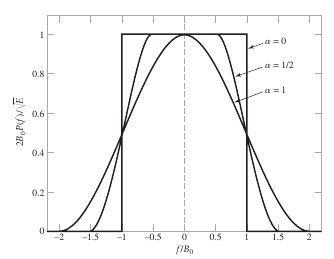
\includegraphics[width=1\linewidth]{img/digital/ISI/MagRRC.png}
        \caption{Espetro RC para vários fatores de \textit{roll-off}.} 
        \label{fig:RRCMag} 
        \vspace{1ex}
    \end{subfigure}%% 
    \begin{subfigure}[b]{0.5\linewidth}
        \centering
        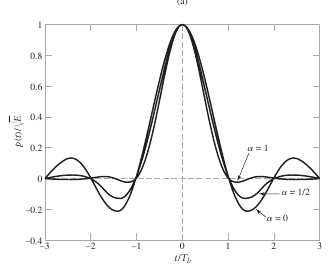
\includegraphics[width=1\linewidth]{img/digital/ISI/TempoRRC.png} 
        \caption{Resposta temporal do pulso.} 
        \label{fig:RRCTempo} 
        \vspace{1ex}
    \end{subfigure} 
    \caption{Pulso Raised Cosine.}
    \label{fig:RRC}
\end{figure}

%//==============================--@--==============================//%
\vspace{-1em}
{
\mdfsetup{linewidth=2pt}

\begin{mdframed}
    $\pmb{\star}$ \textbf{Nota: Transmission Bandwidth Requirement}
    \noindent``(...) The nonzero portion of the raised cosine pulse spectrum P(f) is limited to the interval $(0, 2B_0 - f_1)$ for positive frequencies. Accordingly, the transmission bandwidth required by using the raised cosine pulse spectrum is given by:''\cite{Haykin2007}
    
    $$
        B_t = 2B_0 - f_1 = B_0(1 + \alpha) = \boxed{\dfrac{r_b}{2\log_2(M)}(1 + \alpha)}\qquad (\text{Para códigos NRZ})
    $$

    \noindent Onde $f_v = aB_0$ é a banda adicional (\textit{excess bandwidth}).
\end{mdframed}
}
%//==============================--@--==============================//%
\clearpage
\subsubsection[3.4.3 Eye Pattern]{$\rightarrow$ Eye Pattern}
\label{subsec:EyePattern}

\begin{theo}[\underline{Eye Pattern} \cite{Haykin2007}]{teo/def:nome-unico}\label{teo/def:eyePattern}
    The eye pattern is produced by the synchronized superposition of (as many as possible) successive symbol intervals of the distorted waveform appearing at the output of the receive-filter prior to thresholding.
\end{theo}

\noindent O \textit{Eye Pattern} é uma ferramente de avaliação da qualidade da receção do sinal:
\begin{figure}[H]
    \centering
    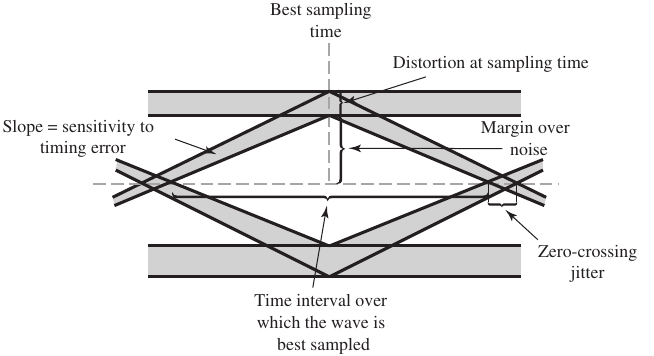
\includegraphics[width = 1\linewidth]{img/digital/ISI/EyePattern.png}
    \caption{Diagrama de Olho.}
    \label{fig:EyePattern}
\end{figure}
%//==============================--@--==============================//%

    \addtocontents{toc}{\protect\newpage}
    \clearpage
    \section{4. Transmissão em canais com AWGN}
        %//==============================--@--==============================//%
\subsection[4.1 Representação geométrica de sinais]{$\rightarrow$ Representação geométrica de sinais}
\label{subsec:geom-representation-of-signals}

A essência da representação geométrica de sinais, é decompor os $M$ sinais de energia, $\{s_i(t)\}$ numa combinação linear de $N$ funções base ortonormais, onde $N \leq M$. Isto é, dado um conjunto de sinais de energia reais, $s_1(t)$, $s_2(t)$, $\dots$, $s_M(t)$ (cada com duração $T$), podemos escrever:
$$
    s_{i}(t) = \sum_{j=1}^{N} s_{ij}\, \phi_j(t),\qquad
    \begin{cases}
        0 \leq t \leq T \\
        i = 1,2,\dots,M
    \end{cases}
$$
em que os coeficientes da expansão são dados por:
$$
    s_{ij} = \int_{0}^{T} s_i(t) \phi_j(t)\, dt,\quad
    \begin{cases}
        i = 1,2,\dots,M \\
        j = 1,2,\dots,N
    \end{cases}
$$
As funções base $\phi_1(t)$, $\phi_2(t)$, $\dots$, $\phi_N(t)$, formam um conjunto ortonormal, i.e.,
$$
    \int_{0}^{T} \phi_i(t) \phi_j(t)\, dt = \delta_{ij} =
    \begin{cases}
        1 & \text{se } i = j \\
        0 & \text{se } i \neq j
    \end{cases}
$$
onde $\delta_{ij}$ é o \textit{Kronecker delta}.

\begin{figure}[H]
    \centering
    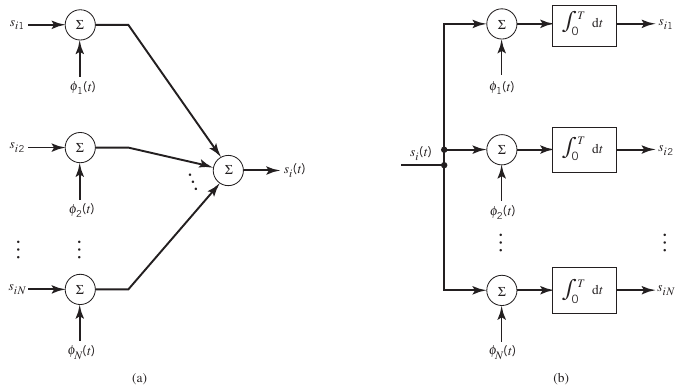
\includegraphics[width = 0.7\linewidth]{img/digital/AWGN-transmission/signals-geom-decomposition.png}
    \caption{(a) Síntese do sinal $s_i(t)$. (b) Análise para construir o vetor sinal $\{s_i\}$.}
    \label{fig:signals-geom-decomposition}
\end{figure}

\noindent Desta forma, é possível representar qualquer sinal do conjunto $\{s_i(t)\}$ sobre um vetor sinal da forma
$$
    \pmb{s}_i = 
    \begin{bmatrix}
        s_{i1}\\
        s_{i2}\\
        \vdots\\
        s_{iN}
    \end{bmatrix},\qquad i = 1,2,\dots,M
$$

\noindent O espaço euclidiano \textit{N-dimensional} onde podemos visualizar estes vetores, é denominado por \textit{signal space}/espaço de sinais.
%//==============================--@--==============================//%
\newpage
\subsubsection[4.1.1 Desigualdade de Schwarz]{$\rightarrow$ Desigualdade de Schwarz}
\label{subsubsec:shwarz}

\begin{mdframed}
Considerando um par de sinais, $s_1(t)$ e $s_2(t)$. A \textit{Desigualdade de Schwarz} afirma que
$$
    \left| \int_{-\infty}^{+\infty} s_1(t)\, s_2^*(t) \, dt \right| \leq \left( \int_{-\infty}^{+\infty} [s_1(t)]^2 \, dt \right)^{1/2}\, \left( \int_{-\infty}^{+\infty} [s_2(t)]^2 \, dt \right)^{1/2}
$$
onde o asterisco ($*$) sobrescrito denota o complexo conjugado. A igualdade apenas se verifica se, e somente se, $s_2(t) = c\, s_1(t)$, onde $c$ é uma constante arbitrária.
\end{mdframed}

%//==============================--@--==============================//%
\subsubsection[4.1.2 Processo de ortogonalização de Gram-Schmidt]{$\rightarrow$ Processo de ortogonalização de Gram-Schmidt}

\begin{theo}[\underline{Gram-Schmidt procedure}]{def:gram-schmidt}\label{def:gram-schmidt}
    Supondo um banco de $M$ sinais de energia, $s_1(t)$, $s_2(t)$, $\dots$, $s_M(t)$. Começamos por escolher um dos sinais ($s_1(t)$ sem perda de generalidade) definimos a primeira base como
    $$
        \phi_1(t) = \frac{s_1(t)}{\sqrt{E_1}}
    $$
    Definem-se em seguida as funções auxiliares
    $$
        g_i(t) = s_i(t) - \sum_{j=1}^{i-1} s_{ij}\, \phi_{j}(t),\qquad s_{ij} = \int_{0}^{T} s_i(t)\phi_j(t) \,dt 
    $$
    tal que as seguintes bases podem ser definidas como
    $$
        \phi_i(t) = \frac{g_i(t)}{\sqrt{\int_{0}^{T} [g_i(t)]^2\, dt}}
    $$
    Repare-se que para $i=1$, $g_i(t)$ reduz-se para $s_i(t)$. Verifica-se sempre que $N \leq M$ (os sinais de energia não são linearmente independentes entre si, ou, no caso limite, todos os sinais de energia são linearmente independentes).
\end{theo}

%//==============================--@--==============================//%
        \clearpage
%//==============================--@--==============================//%
\subsection[4.2 Problema de decisão]{$\rightarrow$ Problema de decisão}
\label{subsec:optimum-receiver-coherent-detection}

Nesta secção é analisado o problema de reconhecer um sinal escolhido aleatoriamente (com probabilidades conhecidas) de um conjunto finito conhecido $\{s_i(t)\}_{i=1}^{M}$ após ser perturbado por um processo de ruído $n(t)$ independente do sinal e adicionado a este. 

Refinadamente, o problema é decidir, qual dos sinais, $s_1(t)$, $s_2(t)$, $\dots$, $s_M(t)$, levou à obtenção do sinal $r(t)$, quando se sabe que $r(t)$ tem a forma
$$
    r(t) = s_i(t) + n(t)
$$
para algum $i$, $1 \leq i \leq M$. Será assumido que $n(t)$ é um processo gaussiano, com densidade espectral de potência $N_0/2$. Os sinais têm energia finita e duração finita. Assume-se que $s_i(t)$, $1 \leq i \leq M$, são definidos num intervalo $0 \leq t \leq T$ e que $r(t)$ é observado no mesmo intervalo. Definimos então o \underline{problema de decisão}.

%//==============================--@--==============================//%
\subsubsection[4.2.1 Caracterização estatística da saída do correlador]{$\rightarrow$ Caracterização estatística da saída do correlador}

Seja $r_j$ definido como
\begin{align*}
    r_j &\delequal \int_{0}^{T} r(t) \phi_j(t)\, dt,\qquad j=1,2,\dots,N \\
    &= s_{ij} + n_{j}
\end{align*}
em que 
$$
    n_j \delequal \int_{0}^{T} n(t) \phi_j(t)\, dt,\qquad j=1,2,\dots,N
$$

\noindent O valor médio do valor observado do processo estocástico é dado por
\begin{align*}
    \mu_{r_j} &= \mathbb{E}[r_j] \\
    &= \mathbb{E}[s_{ij} + n_j] \\
    &= s_{ij} + \mathbb{E}[n_j] = s_{ij}
\end{align*}

\noindent A variância pode ser calculada através da definição
\begin{align*}
    \sigma_{r_j}^2 &= \text{Var}[r_j] \\
    &= \mathbb{E}[(r_j - s_{ij})^2] \\
    &= \mathbb{E}[n_j^2] 
\end{align*}
Desta forma, de acordo com o supramencionado, é possível expandir a expressão como:
\begin{align*}
    \sigma_{r_j}^2 &= \mathbb{E}\left[ \int_{0}^{T} n(t) \phi_j(t)\, dt\, \int_{0}^{T} n(u) \phi_j(u)\, du \right] \\
    &= \int_{0}^{T} \int_{0}^{T} \phi_j(t) \phi_j(u) \mathbb{E}[n(t)n(u)] \, dt\,du
\end{align*}
Dado que 
$$
    \mathbb{E}[n(t)n(u)] = R_{n}(t,u) = \frac{N_0}{2}\, \delta(t-u)
$$
$$
    \therefore \sigma_{r_j}^2 = \frac{N_0}{2} \int_{0}^{T} \phi_j^2(t)\, dt
$$
\begin{theo}[\underline{Teorema da Irrelevância}]{def:irrelevance-theorem}\label{def:irrelevance-theorem}
    Apenas a projeção do ruído nas funções base do conjunto de sinais $\{s_i(t)\}_{i=1}^{M}$ afeta as \textit{estatísticas suficientes} do \underline{problema de decisão}; o restante ruído é irrelevante.
\end{theo}

%//==============================--@--==============================//%
\clearpage
\subsubsection[4.2.2 \textit{Optimum detector}: \textit{M} sinais reais]{$\rightarrow$ \textit{Optimum detector}: $\pmb{M}$ sinais reais no seio do ruído}
Focamo-nos então no problema enunciado no início desta secção, i.e., decidir entre as seguintes $M$ hipóteses
$$
    H_i:\quad y(t) = s_i(t) + n(t),\quad i = 1,2,\dots,M 
$$
após uma observação de $y(t)$ no intervalo de tempo $[0, T]$. Os M sinais $s_i(t)$ são conhecidos e têm energia finita, bem como duração. Através do \hyperref[def:gram-schmidt]{procedimento de Gram-Schmidt}, é possível determinar um conjunto de sinais ortonormais $(\phi_j(t))_{j=1}^{N}$, $N \leq M$, tal que cada $s_i(t)$, $i=1,2,\dots,M$, possa ser representado como uma combinação linear destas bases. Consideremos também uma sequência completa de sinais ortonormais cujos primeiros $N$ elementos são $\phi_1(t)$, $\dots$, $\phi_N(t)$. Denotemos esta sequência por $(\phi_j(t))_{j=1}^{+\infty}$, e definimos
$$
    s_{ij} \delequal \int_{0}^{T} s_i(t)\phi_j(t)\, dt,\quad i=1,2,\dots,M,\quad j=1,2,\dots 
$$
e $n_j$, $Y_j$ do mesmo modo. O \underline{problema de decisão} pode ser formulado da seguinte forma discreta. Escolher entre as $M$ hipóteses
$$
    H_i:\quad (Y_j)_{i=1}^{+\infty} = (s_{i1}+n_1, s_{i2}+n_2, \dots, s_{iN}+n_N, n_{N+1}, n_{N+2},\dots)
$$
$i=1,2,\dots,M$, com base nas observações das VA's $Y_1$, $Y_2$, $\dots$. Dado que as componentes de ruído $n_{N+1}$, $n_{N_2}$,$\dots$, são independentes de $v_1$, $\dots$, $v_N$, e das hipóteses, as observações $Y_{N+1}$, $Y_{N+2}$,$\dots$, não acrescentam informação nenhuma ao processo de decisão. Portanto podemos basear-nos somente na observação de $Y_1$, $Y_2$,$\dots$, $Y_N$. Definindo os vetores linha $[N \times 1]$ $\pmb{Y} \delequal [Y_1,Y_2,\dots,Y_N]$, $\pmb{n} \delequal [n_1,n_2,\dots,n_N]$, e $\pmb{s}_i \delequal [s_{i1},s_{i2},\dots,s_{iN}]$, $i=1,2,\dots,M$, é possível reduzir a decisão para a forma vetorial 
$$
    H_i:\quad \pmb{Y} = \pmb{s}_i + \pmb{n},\quad i=1,2,\dots,M
$$
Desta forma, o \textit{optimum detector} procura funcionar de tal forma que
$$
    \texttt{escolher } H_i \texttt{ se } \pmb{y} \in S_i
$$
onde $\pmb{y}$ denota o valor observado do vetor aleatório $\pmb{Y}$, e $S_1$, $S_2$,$\dots$, $S_M$ são as partições do espaço $N$-dimensional, tal que esta regra dê azo à menor probabilidade de erro média
$$
    P(e) = 1 - \sum_{i=1}^{M} p_i\, \int_{S_i} f_{\pmb{Y}|H_i}\left( \pmb{z} | H_i \right)\, d\pmb{z}
$$
em que $p_i \delequal P\{H_i\}$, $i=1,2,\dots,M$. É verificado que $P(e)$ é minimizado se cada $S_i$ for escolhido de forma a que
$$
    \pmb{z} \in S_i \texttt{ se, e somente se, } p_i\, f_{\pmb{Y} | H_i}(\pmb{z}|H_i) = \max_{j} p_j\, f_{\pmb{Y} | H_j}(\pmb{z}|H_j)
$$
Obtemos então o critério de decisão de \underline{\textit{maximum a posteriori}} (MAP). Neste caso, as $M$ regiões $S_i$ são denominadas por \textit{regiões de decisão} MAP. No caso especial em que as hipóteses $H_i$ são equiprováveis, i.e., $p_i = 1/M$, obtém-se
$$
    \pmb{z} \in S_i \texttt{ se, e somente se, } f_{\pmb{Y} | H_i}(\pmb{z}|H_i) = \max_{j} f_{\pmb{Y} | H_j}(\pmb{z}|H_j)
$$
que corresponde à regra de decisão de \underline{\textit{máxima verosimilhança}} (ML). Apesar de apenas minimizar $P(e)$ para hipóteses $H_i$ equiprováveis, é o método de deteção mais utilizado, e será onde confinaremos a nossa deteção.

Definindo a hipótese auxiliar
$$
    H_0:\quad \pmb{Y} = \pmb{n},
$$
a condição de ML pode ser reescrita como
$$
    \pmb{z} \in S_i \texttt{ se, e somente se, } \Lambda_i(\pmb{z}) = \max_{i} \Lambda_j(\pmb{z})
$$
onde definimos os \textit{likelihood ratios}
$$
    \Lambda_i(\pmb{z}) \delequal \frac{f_{\pmb{Y} | H_i}(\pmb{z}|H_i)}{f_{\pmb{Y} | H_0}(\pmb{z}|H_0)}
$$
Deste modo, a regra de decisão ML é
$$
    \texttt{escolher } H_i \texttt{ se } \Lambda_i(\pmb{y}) = \max_{i} \Lambda_j(\pmb{y})
$$
onde $\pmb{y}$ representa, como anteriormente, o valor observado de $\pmb{Y}$. Isto é, o detetor ML calcula os $M$ \textit{likelihood ratios} $\Lambda_1(\pmb{y})$, $\Lambda_2(\pmb{y})$,$\dots$,$\Lambda_M(\pmb{y})$, e escolhe a hipótese que corresponde ao maior de entre a seleção. Observando que $pmb{Y}$ é um vetor aleatório gaussiano com valor médio $\pmb{s}_i$ (ou zero, para $i=0$), componentes independentes, e variância $N_0/2$ para cada componente, temos, para $i=1,2,\dots,M$,
$$
    \Lambda_i(\pmb{z}) = \frac{\exp[-(1/N_0)\, |\pmb{y}-\pmb{s}_i|^2]}{\exp[-(1/N_0)\, |\pmb{y}|^2]}
$$
onde $|\pmb{x}|^2 = \pmb{x}\pmb{x}^T = \sum_{j=1}^{N} x^2_j$ (módulo ao quadrado do vetor $\pmb{x}$). Definindo os \textit{log-likelihood ratios}
$$
    \lambda_i(\pmb{y}) \delequal \ln{\Lambda_i(\pmb{y})}
$$
permite reduzir a condição para a simples forma
$$
    \texttt{escolher } H_i \texttt{ se } \pmb{y}\pmb{s}_i^T - \frac{1}{2} |\pmb{s}_i|^2 = \max_{i}\left\{ \pmb{y}\pmb{s}_j^T - \frac{1}{2} |\pmb{s}_j|^2 \right\} 
$$
Uma expressão mais familiar para o \textit{log-likelihood ratio} pode ser dada por 
\begin{mdframed}
$$
    \therefore \lambda_i(y) = \frac{2}{N_0} \int_{0}^{T} y(t) s_i(t)\, dt - \frac{1}{N_0} \int_{0}^{T} s_i^2(t)\, dt,\qquad i=1,2,\dots,M
$$
\end{mdframed}

\begin{figure}[ht] 
    \begin{subfigure}[b]{0.5\linewidth}
        \centering
        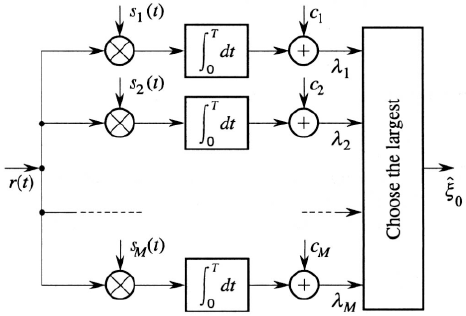
\includegraphics[width=0.9\linewidth]{img/digital/AWGN-transmission/detection-correlator.png}
        \caption{Implementação com $M$ correladores.} 
        \label{fig:detection-correlator} 
    \end{subfigure}%%
    \begin{subfigure}[b]{0.5\linewidth}%%
        \centering
        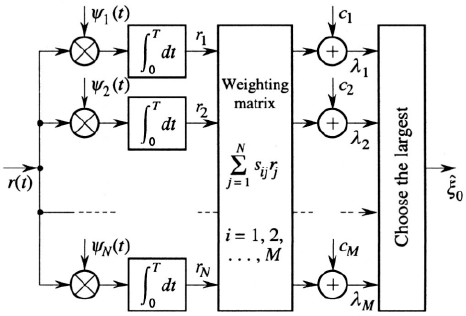
\includegraphics[width=0.9\linewidth]{img/digital/AWGN-transmission/detection-reference.png} 
        \caption{Redução de complexidade, $N \leq M$.} 
        \label{fig:detection-reference} 
    \end{subfigure}
    \caption{Implementação do recetor ótimo coerente com correladores.\cite{Benedetto1999}}
    \label{fig:} 
\end{figure}

\noindent Em que as constantes $c_i$, $i=1,2,\dots,M$, são dadas por
$$
    c_i \delequal -\frac{1}{2} \int_{0}^{T} s_i^2(t)\, dt = -\frac{1}{2} E_i
$$
onde $E_i$ denota a energia do $i$-ésimo sinal.
%Adoro-te :3
%//==============================--@--==============================//%
        %//==============================--@--==============================//%
\clearpage
\subsection[4.3 Filtro adaptado]{$\rightarrow$ Filtro adaptado}
\label{subsec:matched-filter}

\begin{theo}[\underline{Matched filter}]{def:matched-filter}\label{def:matched-filter}
    $$
        h(t) \delequal \alpha s(T-t)\; \xrightleftharpoons[]{\mathcal{F}}\; H(f) \delequal \alpha S^*(f)e^{-j2\pi f T},\qquad \alpha \in \mathbb{R}
    $$

    \noindent $\pmb{\rightarrow}$ \textbf{Nota:} 
    $$
        r(t) \ast h(t)\biggr|_{t=T} = \int_{0}^{T} r(\tau)h(T-\tau) \,dt =  \int_{0}^{T} r(\tau)s(\tau) \,dt
    $$
    Então, um filtro adaptado\footnotemark[3] cujo \textit{output} é amostrado no instante $T$ extrai do sinal observado $r(t)$ as estatísticas suficientes para o problema da decisão.

    \vspace{-1em}
    \begin{figure}[H]
        \centering
        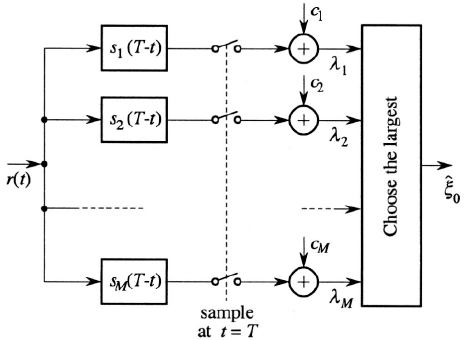
\includegraphics[width=0.5\linewidth]{img/digital/AWGN-transmission/detection-matched-filter.png} 
        \caption{Implementação do recetor ótimo coerente com filtros adaptados.\cite{Benedetto1999}} 
        \label{fig:detection-matched-filter} 
    \end{figure}
\end{theo}

\noindent Uma propriedade do filtro adaptado é que maximiza o SNR à saída. Quando a entrada do filtro é a soma do sinal $s(t)$ com ruído $n(t)$, no instante $t=T$, a sua saída será composta por dois termos: a primeira parte é respetiva ao sinal
$$
    \int_{-\infty}^{+\infty} H(f) S(f) e^{j2\pi f T} \,df,
$$
onde $H(f)$ representa a função de transferência do filtro; a segunda é respetiva à parte do ruído, uma VA gaussiana com média $\mu$ nula e variância dada por
$$
    \sigma^2 = \frac{N_0}{2}\int_{-\infty}^{+\infty} |H(f)|^2 \,df
$$
Se definirmos o SNR à saída do filtro como
$$
    \zeta^2 \delequal \dfrac{\displaystyle \left[ \int_{-\infty}^{+\infty} H(f) S(f) e^{j2\pi f T} \,df \right]^2}{\displaystyle \frac{N_0}{2}\, \int_{-\infty}^{+\infty} |H(f)|^2 \,df}
$$
É possível demostrar que tem o valor máximo para \underline{filtro adaptado}. Invocando a \hyperref[subsubsec:shwarz]{\underline{Desigualdade de Schwarz}} ($A = \alpha B^*$):
\vspace{-1em}
$$
    \rightarrow \left| \int_{\mathbb{R}} A\, B^* \right|^2 \leq \int_{\mathbb{R}} |A|^2\; \int_{\mathbb{R}} |B|^2
    \implies
    \zeta^2 \leq \frac{\displaystyle \cancel{\int_{\mathbb{R}} |H(f)|^2 \,df}\; \int_{\mathbb{R}} |S(f)|^2 \,df}{\displaystyle \frac{N_0}{2} \cancel{\int_{\mathbb{R}} |H(f)|^2 \,df}}
    = \frac{2 E_s}{N_0}
$$
\vspace{-1em}%adoro-te
$$
    \boxed{%
        \therefore \text{PSNR} \delequal \frac{2E_s}{N_0}
    }
$$
\footnotetext[3]{Para sinais pares, o filtro adaptado é uma réplica deslocada do pulso de entrada.}
%//==============================--@--==============================//%

    \clearpage
    \section{5. Técnicas de Modelação Digital (banda passante)}
        %\clearpage
%//==============================--@--==============================//%
\subsection[5.1 ASK (\textit{Amplitude-Shift Keying})]{$\rightarrow$ ASK (\textit{Amplitude-Shift Keying})}
\label{subsec:M-ASK}

\begin{mdframed}
Uma sequência $\xi$ de $K$ símbolos é transportada pelo sinal
$$
    v_\xi(t) = \mathbb{R}e\mathbb{e}\left\{ \sum_{k=0}^{K-1} \xi_k\, s(t-kT) \right\},\quad 0 \leq t \leq KT
$$
em que as variáveis aleatórias $\xi_k$ tomam valores no conjunto de amplitudes equi-espaçadas $\left\{ a_i \right\}_{i=1}^{M}$, dadas por (código polar e unipolar respetivamente)
$$
    a_i = (2i - 1 - M)\,\frac{d}{2} \;\lor\; a_i = (2i-M)\,d,\quad i = 1,2,\dots,M
$$
Consequentemente, as formas de onda utilizadas pelo modulador são somente múltiplos escalares de uma única onda. Se $s(t)$ for um pulso de energia unitária, representa um sinal base da expansão ortonormada, o que leva à conclusão de que o sinal conjunto, é \underline{uni-dimensional}.
\end{mdframed}
%//==============================--@--==============================//%
\subsubsection[5.1.1 Probabilidade de erro (código polar)]{$\rightarrow$ Probabilidade de erro (código polar)}
{\small
A probabilidade de erro de símbolo da ASK para uma deteção coerente, pode ser aferida explicitamente se a probabilidade de uma decisão correta for conhecida
$$
    P(c) = \frac{1}{M}[2q_1 + (M-2)q_2]
$$
em que $q_1$ é a probabilidade da decisão correta para os dois pontos exteriores da constelação, e $q_2$ é a probabilidade de decisão correta para os restantes $(M-2)$ pontos interiores. Definindo
$$
    p = \frac{1}{2}\, \text{erfc}\left(\frac{d}{2\sqrt{N_0}}\right)
$$
temos que $q_1 = 1 - p$ e $q_2 = 1 - 2p$. Assim,
$$
    P(c) = 1 - 2p\frac{M-1}{M}
$$
e finalmente
$$
    P(e) = \frac{M-1}{M}\, \text{erfc}\left(\frac{d}{2\sqrt{N_0}}\right).
$$
Para exprimir $P(e)$ em função de $E$, aproveita-se o facto de que a energia média\footnotemark[4] do símbolo é dada por
$$
    E = \frac{1}{M} \sum_{i=1}^{M} a_i^2 = \frac{d^2}{4M} \sum_{i=1}^{M} (2i - 1 - M)^2 = \frac{M^2-1}{12}\, d^2
$$
Então, dado que $E = \log_2(M)\, E_b$,
$$
    \therefore P(e) = \frac{M-1}{M}\, \text{erfc}\left( \sqrt{\frac{3\log_2(M)}{M^2-1}\frac{E_b}{N_0}} \right)
$$
}
\renewcommand*{\thefootnote}{\fnsymbol{footnote}}
\footnotetext[4]{%
    A \textit{power efficiency} assintótica é o factor multiplicativo de $E_b/N_0$ no argumento da $\text{erfc}(\cdot)$. Assim,
    $$
        \gamma_{\text{ASK}} = \frac{3\log_2(M)}{M^2-1} 
    $$
    que se verifica decrescente para valores de $M$ cada vez maiores.
}
\renewcommand*{\thefootnote}{\arabic{footnote}}

\footnotetext[4]{%
    Em PAM/ASK, a energia média transmitida difere da \textit{peak energy} $E_p = (M-1)^2 d^2/4$, que é a energia do sinal de máxima amplitude. Verifica-se que $E_p/E = 3 (M-1)/(M+1)$.
}
%//==============================--@--==============================//%
\subsubsection[5.1.2 Probabilidade de erro (código unipolar)]{$\rightarrow$ Probabilidade de erro (código unipolar)}
{\small
Partindo novamente de 
$$
    P(e) = \frac{M-1}{M}\, \text{erfc}\left( \frac{d}{2\sqrt{N_0}} \right)
$$
Neste caso o valor da energia média do símbolo é dada por
$$
    E = \frac{1}{M} \sum_{i+1}^{M} a_i^2 = \frac{d^2}{4M} \sum_{i+1}^{M} (2i-M)^2 = \frac{M^2+2}{12}d^2
$$
Desta forma
$$
    P(e) = \frac{M-1}{M}\, \text{erfc}\left( \sqrt{\frac{3 \log_2(M)}{M^2+2} \frac{E_b}{N_0}} \right)
$$
}
%//==============================--@--==============================//%
\subsubsection[5.1.3 Espectro de potência e eficiência espectral]{$\rightarrow$ Espectro de potência e eficiência espectral}

A densidade espectral de potência do sinal ASK $v_\xi(t)$ é dada por
$$
    S_{v_\xi}(f) = \frac{E}{T}\left|S(f)\right|^2
$$
onde $S(f)$ denota a Transformada de Fourier de $s(t)$.

\vspace{0.5em}
\noindent A largura de banda de Shannon para esta modulação é $W = 1/2T$, e então, a eficiencia espectral é dada por
$$
    \left(\frac{R_s}{W}\right)_{\text{ASK}} = 2 \log_2(M)
$$

\vspace{0.5em}
\noindent Conclui-se que para ASK, ao aumentar o valor de $M$ ocorre uma melhoria da eficiência espectral, no entanto, ocorre também uma diminuição da \textit{power efficiency}.
%//==============================--@--==============================//%
        \clearpage
%//==============================--@--==============================//%
\subsection[5.2 PSK (\textit{Phase-Shift Keying})]{$\rightarrow$ PSK (\textit{Phase-Shift Keying})}
\label{subsec:M-PSK}
\begin{mdframed}
Uma sequência $\xi$ de $K$ símbolos é transportada pelo sinal
$$
    v_\xi(t) = \mathbb{R}e\left\{ \sum_{k=0}^{K-1} \xi_k\, s(t-kT) e^{j2\pi f_c t} \right\},\quad 0 \leq t \leq KT
$$
onde $\xi_k = e^{j\phi_k}$, e cada fase discreta $\phi_k$ toma valores no conjunto
$$
    \left\{ \frac{2\pi}{M}(i-1) + \Phi \right\}_{i=1}^{M}
$$
em que $\Phi$ é uma constante de fase arbitrária. Assume-se que a forma de onda do modulador é retangular, i.e., $s(t) \equiv u_T(t)$ um pulso retangular de amplitude A e duração T, de tal forma que o envelope do sinal PSK seja constante (são possíveis outras formas de onda, mas assumimos esta). Podemos escrever explicitamente
\begin{align*}
    v_\xi(t) &= A\sum_{k=0}^{K-1} u_T(t-kT)\cos(2\pi f_c t + \phi_k) = \\
    &= I(t) \cos(2\pi f_c t) - Q(t) \sin(2\pi f_c t)
\end{align*}
definimos então as componentes em fase e em quadratura do sinal PSK:
$$
    I(t) \delequal A\sum_{k=0}^{K-1} \cos(\phi_k) u(t-kT)
$$
$$
    Q(t) \delequal A\sum_{k=0}^{K-1} \sin(\phi_k) u(t-kT)
$$
\end{mdframed}
%//==============================--@--==============================//%
\vspace{-1em}
\subsubsection[5.2.1 Probabilidade de erro]{$\rightarrow$ Probabilidade de erro}
Na forma geral, para um sinal $M$-PSK, podemos definir os limites superiores e inferiores de $P(e)$. Aqui $E_b = E/\log_2(M)$, e então, temos
$$
    \frac{1}{2}\, \text{erfc}\left( \sqrt{\frac{E_b}{N_0}\log_2(M)} \sin{\frac{\pi}{M}} \right) \leq P(e) \leq \text{erfc}\left( \sqrt{\frac{E_b}{N_0}\log_2(M)} \sin{\frac{\pi}{M}} \right)
$$

\renewcommand*{\thefootnote}{\fnsymbol{footnote}}
\footnotetext[4]{%
    A \textit{power efficiency} assintótica da modulação PSK é 
    $$
        \gamma_{\text{PSK}} = \sin^2\left(\frac{\pi}{M}\right) \cdot \log_2(M) 
    $$
    que se verifica decrescente para valores de $M$ cada vez maiores.
}
\renewcommand*{\thefootnote}{\arabic{footnote}}
%//==============================--@--==============================//%
\vspace{-1em}
\subsubsection[5.2.2 Espectro de potência e eficiência espectral]{$\rightarrow$ Espectro de potência e eficiência espectral}

A densidade espectral de potência do sinal PSK é dada por
$$
    S_{v_\xi}(f) = \frac{1}{4}[S(-f-f_0) + S(f-f_0)]
$$
onde $S(f)$ representa a Transformada de Fourier de $s(t)$ (\textit{vide} secção sobre \hyperref[teo/def:LineCodes]{código de linha}).

\vspace{0.5em}
\noindent Dado que $N=2$, a largura de banda de Shannon para esta modulação é $W = 1/T$, e então, a eficiencia espectral é dada por
$$
    \left(\frac{R_s}{W}\right)_{\text{ASK}} = \log_2(M)
$$

\vspace{0.5em}
\noindent Conclui-se que para PSK, ao aumentar o valor de $M$ ocorre também melhoria na eficiência da largura de banda, verifica-se uma diminuição da \textit{power efficiency}.

%//==============================--@--==============================//%
\newpage
\subsubsection[5.2.3 Exercícios]{$\pmb{\rightarrow}$ Exercícios}
\paragraph[5.2.3.1 Oscilador com erro de fase]{$\pmb{\star}$ Considere um sistema PSK binário com formas de onda equiprováveis $\pmb{s_1(t) = \cos(2\pi f_c t) = -s_2(t)}$. No detetor de filtro adaptado a referência é $\pmb{\cos(2\pi f_c t + \phi)}$, em que $\pmb{\phi}$ é um erro de fase. Calcule a probabilidade de erro de bit.}\mbox{}\\

\noindent Partindo de 
$$
    r(t) = s_i(t) + n(t)\quad\land\quad s_i(t) = \pm \cos(2\pi f_c t),\quad i = 1,2
$$

\begin{align*}
    \rightarrow \int _{0}^{T_b} \cos(2\pi f_c t) \cos(2\pi f_c t + \phi)\, dt &= \int _{0}^{T_b} \cos(2\pi f_c t) \left[ \cos(2\pi f_c t)\cos(\phi) - \sin(2\pi f_c t)\sin(\phi) \right]\, dt = \\
    &= \int _{0}^{T_b} \left[ \cos(2\pi f_c t)\right]^2 \cos(\phi)\, dt - 0 = \\
    &= \frac{1}{2}\cos(\phi)\, T_b
\end{align*}

\vspace{0.75em}
\noindent $\rightarrow r_1 = s_{11} + n_1$ com $\mathbb{E}[r_1] = 1/2 \cos(\phi)\, T_b$, dado que $\mathbb{E}[n_1]$ (valor esperado de um processo gaussiano) é nulo.
\begin{align*}
    \sigma^2_{r_1} &= \mathbb{E}[(r_1 - \mu)^2] = \mathbb{E}[n_1^2] = \\
    &= \mathbb{E}\left[ \int_{0}^{T_b} n(t) \cos(2\pi f_c t + \phi) \, dt\; \int_{0}^{T_b} n(u) \cos(2\pi f_c u + \phi) \, du \right] = \\
    &= \int_{0}^{T_b} \int_{0}^{T_b} \cos(2\pi f_c u + \phi) \cos(2\pi f_c t + \phi)\, \mathbb{E}[n(t) n(u)] \, du\, dt = \\
    &= \int_{0}^{T_b} \int_{0}^{T_b} \cos(2\pi f_c u + \phi) \cos(2\pi f_c t + \phi)\, R_n(t,u)\, du\, dt = \\
    &= \frac{N_0}{2} \int_{0}^{T_b} \int_{0}^{T_b} \cos(2\pi f_c u + \phi) \cos(2\pi f_c t + \phi)\, \delta(t-u)\, du\, dt = \\
    &= \frac{N_0}{2} \int_{0}^{T_b} \left[\cos(2\pi f_c u + \phi)\right]^2\, du = \\
    &= \frac{N_0}{2} \int_{0}^{T_b} \left[ \frac{1}{2} + \frac{1}{2}\cos(4\pi f_c u + 2\phi) \right]\, du = \frac{N_0 T_b}{4} + \frac{N_0}{4}\int_{0}^{T_b} \cos(4\pi f_c u + 2\phi)\, du = \\
    &= \frac{N_0 T_b}{4} + \frac{N_0}{4} \int_{2\phi}^{4\pi f_c T_b + 2\phi} \cos(x)\, \frac{dx}{4\pi f_c} = \frac{N_0 T_b}{4} + \frac{N_0}{16\pi f_c}\; \cancelto{0,\, \because \textit{bandpass}}{\Bigr[\sin(x)\Bigr]_{2\phi}^{4\pi f_c T_b + 2\phi}} = \\
    &= \frac{N_0 T_b}{4}
\end{align*}

\vspace{0.75em}
\noindent Dado que as formas de onda são equiprováveis e antipodais
$$
    \therefore \frac{1}{2}\, \text{erfc}\left(\frac{d/2}{\sqrt{2}\sigma}\right) = \frac{1}{2}\, \text{erfc}\left(\frac{1/2 \cos(\phi)\, T_b}{\sqrt{2}\sqrt{N_0 T_b/4}}\right) = \frac{1}{2} \, \text{erfc}\left( \sqrt{\frac{E_b}{N_0}} \cos(\phi) \right)
$$

\vspace{0.75em}
\noindent $\pmb{\rightarrow}$ \textbf{Notas:} 
$$R_n(t,u) = N_0/2 \cdot \delta(t-u)$$
$$E_b = \int_{0}^{T_b} [s_1(t)]^2\, dt = T_b/2$$
        \clearpage
%//==============================--@--==============================//%
\subsection[5.3 QAM (\textit{Quadrature Amplitude Modulation})]{$\rightarrow$ QAM (\textit{Quadrature Amplitude Modulation})}
\label{subsec:M-QAM}

\begin{mdframed}
    Este é um esquema linear, em que os símbolos determinam a amplitude e a fase do sinal portadora. Ao contrário do esquema PSK, o envelope não é constante. Uma sequência $\xi$ de $K$ símbolos é representada pelo sinal
    $$
        v_{\xi}(t) = \mathbb{R}e\left\{ \sum_{k=0}^{K-1} \xi_k s(t-kT) e^{j2\pi f_0 t} \right\},\quad 0 \leq t \leq KT
    $$
    em que a VA discreta $\xi_k$ é definida como
    $$
        \xi_k \delequal \xi_k^{'} + \xi_k^{''} = A_k e^{j\phi_k} 
    $$
    e $s(t)$ é um sinal de banda base complexo de duração $T$. No caso de $s(t) = u_T(t)$, podemos reescrever a expressão como
    $$
         v_{\xi}(t) = \sum_{k=0}^{K-1} \{ \xi_k^{'} \cos(2\pi f_0 t) - \xi_k^{''} \sin(2\pi f_0 t) \} u_T(t)
    $$
    que exprime o sinal transmitido na forma de uma série de portadoras---par ortogonal---moduladas pelo conjunto de amplitudes discretas. Esta família de constelações do sinal é bi-dimensional, e o modulador e desmodulador tomam a mesma estrutura do PSK. 
\end{mdframed}

%//==============================--@--==============================//%
\subsubsection[5.3.1 Probabilidade de erro]{$\rightarrow$ Probabilidade de erro}

Um limite superior fácil para a $P(e)$ (útil para valores altos de $M$, e $E_b/N_0$ muito grandes), pode ser obtida por 
$$
    P(e) \leq 2\, \text{erfc}\left( \sqrt{\frac{3 \log_2(M)}{2(M-1)}\frac{E_b}{N_0}} \right)
$$
em que 
$$
    E = \frac{M-1}{6}\, d^2
$$

\renewcommand*{\thefootnote}{\fnsymbol{footnote}}
\footnotetext[4]{%
    A \textit{power efficiency} assintótica da modulação QAM é 
    $$
        \gamma_{\text{QAM}} = \frac{3}{2} \frac{\log_2(M)}{M-1}
    $$
    que se verifica decrescente para valores de $M$ cada vez maiores.
}
\renewcommand*{\thefootnote}{\arabic{footnote}}

%//==============================--@--==============================//%
\subsubsection[5.3.2 Espectro de potência e eficiência espectral]{$\rightarrow$ Espectro de potência e eficiência espectral}

A densidade espectral de potência do sinal QAM é dada por
$$
    S_{v_\xi}(f) = \frac{\mathbb{E}[|\xi_k|^2]}{T}\left|\tilde{S}(f)\right|^2
$$
em que $\tilde{S}(f)$ denota a Transformada de Fourier do sinal complexo $\tilde{s}(t)$.

\vspace{0.5em}
\noindent Dado que $N=2$, a largura de banda de Shannon para esta modulação é $W = 1/T$, e então, a eficiencia espectral é dada por (igual a PSK)
$$
    \left(\frac{R_s}{W}\right)_{\text{ASK}} = \log_2(M)
$$

\vspace{0.5em}
\noindent Conclui-se que para QAM, ao aumentar o valor de $M$ ocorre uma melhoria na eficiência da largura de banda, no entanto, ocorre também uma diminuição da \textit{power efficiency}.

%//==============================--@--==============================//%
\newpage
\subsubsection[5.3.3 Exercícios]{$\pmb{\rightarrow}$ Exercícios}
\paragraph[5.3.3.1 ]{$\pmb{\star}$ }\mbox{}\\



%//==============================--@--==============================//%
        \clearpage
%//==============================--@--==============================//%
\subsection[5.4 FSK (\textit{Frequency-Shift Keying})]{$\rightarrow$ FSK (\textit{Frequency-Shift Keying})}
\label{subsec:M-FSK}

\begin{mdframed}
    Este é um esquema de modulação não linear em que os símbolos fonte determinam a frequência de uma portadore de envelope constante. Especificamente, assume-se que o modulador consiste num conjunto de $M$ osciladores sintonizados às frequências desejadas. 

    Uma sequência de $K$ símbolos é representada pelo sinal
    $$
    v_\xi(t) = \mathbb{R}e\left\{ \sum_{k=0}^{K-1} s(t-kT) e^{j2\pi f_d \xi_k(t-kT)} e^{j2\pi f_c t} \right\},\quad 0 \leq t \leq KT
    $$
    onde as VA's discretas $\xi_k$ tomam valores no conjunto $\{2i-1-M\}_{i=1}^{M}$, e portanto, $2f_d$ é a separação entre frequências adjacentes.

    O transmissor utiliza os sinais
    \begin{align*}
        s_i(t) &= A \cos(2\pi f_i t), \qquad\qquad\quad\; 0 \leq t \leq T \\
        f_i &= f_c + (2i-1-M)f_d, \qquad i = 1,2,\dots,M 
    \end{align*}
    que têm energia comum, $E=A^2T/2$, e um envelope constante.

    \vspace{0.75em}
    \noindent Os sinais podem ser feitos ortogonais, ao escolher uma separação de frequências apropriada. Temos,
    \begin{align*}
        \int_{0}^{T} s_n(t) s_m(t)\, dt &= A^2 \int_{0}^{T} \cos(2\pi f_n t) \cos(2\pi f_m t) \, dt \\
        &= \frac{A^2}{2} \int_{0}^{T} \cos(2\pi[f_n + f_m]t)\, dt +  \frac{A^2}{2} \int_{0}^{T} \cos(2\pi[f_n - f_m]t)\, dt \\
        &= \cancel{\frac{A^2 T}{2} \frac{\sin(2\pi [f_n + f_m] T)}{2\pi [f_n + f_m] T}} + \frac{A^2 T}{2} \frac{\sin(2\pi [f_n - f_m] T)}{2\pi [f_n - f_m] T} \\
        &= \frac{A^2 T}{2} \frac{\sin(4\pi [n - m]f_d T)}{4\pi [n - m]f_d T}
    \end{align*}
    Assumimos que o produto $f_c T$ da frequência da portadora e do intervalo de símbolo é tão grande que o primeiro termo da expressão anterior pode ser descartado (\textit{bandpass assumption}). Desta forma, o produto escalar das duas formas de onda é nulo quando $4\pi f_d T$ é um multiplo não nulo de $\pi$. A menor separação que produz um par de sinais ortogonais é
    $$
        2 f_d = \frac{1}{2T}
    $$
\end{mdframed}

%//==============================--@--==============================//%
\subsubsection[5.4.1 Probabilidade de erro]{$\rightarrow$ Probabilidade de erro}

Com base na \textit{union bound}, temos o seguinte limite superior para a probabilidade de erro de símbolo
$$
    P(e) \leq \frac{M-1}{2}\, \text{erfc}\left( \sqrt{\frac{\log_2(M)}{2}\frac{E_b}{N_0}} \right)
$$

\renewcommand*{\thefootnote}{\fnsymbol{footnote}}
\footnotetext[4]{%
    A \textit{power efficiency} assintótica da modulação FSK é 
    $$
        \gamma_{\text{FSK}} = \frac{1}{2} \log_2(M)
    $$
    que, ao contrário das modulações previamente observadas, se verifica \underline{crescente} para valores de $M$ cada vez maiores.
}
\renewcommand*{\thefootnote}{\arabic{footnote}}

%//==============================--@--==============================//%
\newpage
\subsubsection[5.4.2 Espectro de potência e eficiência espectral]{$\rightarrow$ Espectro de potência e eficiência espectral}

O espectro de potência é dado por
$$
    \pmb{\dots}
$$

\vspace{0.75em}
Neste caso, $N=M$, portanto a largura de banda de Shannon deste esquema de modulação é $W=M/2T$, e a sua eficiência espectral é dada por
$$
    \left(\frac{R_s}{W}\right)_{\text{FSK}} = 2\frac{\log_2(M)}{M}
$$
Note-se que ao contrário dos esquemas anteriores (ASK, PSK e QAM), ao aumentar $M$, a eficiência espectral do FSK ortogonal \underline{diminui}. Por outro lado, a \textit{power efficiency} aumenta.

%//==============================--@--==============================//%
\subsubsection[5.4.3 Exercícios]{$\pmb{\rightarrow}$ Exercícios}
\paragraph[5.4.3.1 ]{$\pmb{\star}$ }\mbox{}\\


%//==============================--@--==============================//%

    %% refs
    \clearpage
    \bibliographystyle{unsrtnat}
    \nocite{*}
    {\footnotesize%
    \bibliography{refs}}
    %% attachments
    %\newpage
    %\input{appendix.tex}

\end{document}%